%%
%% This is file `sample-acmsmall.tex',
%% generated with the docstrip utility.
%%
%% The original source files were:
%%
%% samples.dtx  (with options: `acmsmall')
%% 
%% IMPORTANT NOTICE:
%% 
%% For the copyright see the source file.
%% 
%% Any modified versions of this file must be renamed
%% with new filenames distinct from sample-acmsmall.tex.
%% 
%% For distribution of the original source see the terms
%% for copying and modification in the file samples.dtx.
%% 
%% This generated file may be distributed as long as the
%% original source files, as listed above, are part of the
%% same distribution. (The sources need not necessarily be
%% in the same archive or directory.)
%%
%%
%% Commands for TeXCount
%TC:macro \cite [option:text,text]
%TC:macro \citep [option:text,text]
%TC:macro \citet [option:text,text]
%TC:envir table 0 1
%TC:envir table* 0 1
%TC:envir tabular [ignore] word
%TC:envir displaymath 0 word
%TC:envir math 0 word
%TC:envir comment 0 0
%%
%%
%% The first command in your LaTeX source must be the \documentclass
%% command.
%%
%% For submission and review of your manuscript please change the
%% command to \documentclass[manuscript, screen, review]{acmart}.
%%
%% When submitting camera ready or to TAPS, please change the command
%% to \documentclass[sigconf]{acmart} or whichever template is required
%% for your publication.
%%
%%
\documentclass[acmsmall,manuscript,screen,review,anonymous]{acmart}

%%
%% \BibTeX command to typeset BibTeX logo in the docs
\AtBeginDocument{%
  \providecommand\BibTeX{{%
    Bib\TeX}}}

%% Rights management information.  This information is sent to you
%% when you complete the rights form.  These commands have SAMPLE
%% values in them; it is your responsibility as an author to replace
%% the commands and values with those provided to you when you
%% complete the rights form.
\setcopyright{acmcopyright}
\copyrightyear{2018}
\acmYear{2018}
\acmDOI{XXXXXXX.XXXXXXX}


%%
%% These commands are for a JOURNAL article.
\acmJournal{JACM}
\acmVolume{37}
\acmNumber{4}
\acmArticle{111}
\acmMonth{8}

%%
%% Submission ID.
%% Use this when submitting an article to a sponsored event. You'll
%% receive a unique submission ID from the organizers
%% of the event, and this ID should be used as the parameter to this command.
%%\acmSubmissionID{123-A56-BU3}

%%
%% For managing citations, it is recommended to use bibliography
%% files in BibTeX format.
%%
%% You can then either use BibTeX with the ACM-Reference-Format style,
%% or BibLaTeX with the acmnumeric or acmauthoryear sytles, that include
%% support for advanced citation of software artefact from the
%% biblatex-software package, also separately available on CTAN.
%%
%% Look at the sample-*-biblatex.tex files for templates showcasing
%% the biblatex styles.
%%

%%
%% The majority of ACM publications use numbered citations and
%% references.  The command \citestyle{authoryear} switches to the
%% "author year" style.
%%
%% If you are preparing content for an event
%% sponsored by ACM SIGGRAPH, you must use the "author year" style of
%% citations and references.
%% Uncommenting
%% the next command will enable that style.
%%\citestyle{acmauthoryear}

% Comments
\newcommand{\mycomment}[2]{{\small\color{magenta}\underline{\sf{#1}}:} {\color{magenta}{\small #2}}}
\newcommand{\todo}[1]{\mycomment{Todo}{#1}}
\newcommand{\gcmt}[1]{\mycomment{Guan}{#1}}

% Shorthand
\newcommand{\Da}{\Downarrow}

% Unicode char
\usepackage{newunicodechar}
\newunicodechar{λ}{\lambda}
\newunicodechar{Σ}{\Sigma}
\newunicodechar{ρ}{\rho}
\newunicodechar{σ}{\sigma}
\newunicodechar{τ}{\tau}

% Semantics and reserved words
\mathchardef\mhyphen="2D
\usepackage[inference,ligature,reserved,shorthand]{semantic}
\reservestyle[\mathinner]{\command}{\mathit}
\command{let, in}
\command{true, false, bool, int, unit}
\command{pair, fst, snd, as}
\command{and, or, not, nand, nor, xor, for}
\command{if, then, else, while, print, fix, ref, var, when, do, end, robot, whereAmI, left, right, up, down}
\command{andf[and_f], andfp[and_f']}
\command{halfa[half\mhyphen adder], fulla[full\mhyphen adder], Rf[Ref]}

\reservestyle[\mathinner]{\Constructor}{\mathbf}
\Constructor{Bool, True, False}
\Constructor{Int, Lit, Plus, Eq, Lt}
\Constructor{Abs, App, Loc, Ref}

% Macro for Osazone semantics
\NewDocumentCommand{\branch}{ >{\SplitList{&}} m }{%
  \left(\begin{aligned} %
      \ProcessList{#1}{\brfunc}%
    \end{aligned}\right)%
}

\NewDocumentCommand{\brfunc}{m}{%
  & #1%
}

\newcommand{\lt}{\mathbf{let}}
\newcommand{\monad}{\mathbf{monad}~}
\newcommand{\as}{~\mathbf{as}~}

\newcommand{\Let}[2]{\lt~#1=#2;~}

\newcommand{\Exp}{\mathit{Exp}}
\newcommand{\Type}{\mathit{Type}}
\newcommand{\Id}{\mathit{Id}}
\newcommand{\Int}{\mathit{Int}}
\newcommand{\newLoc}{\mathit{newLoc}}
\newcommand{\store}{\mathit{store}}
\newcommand{\fetch}{\mathit{fetch}}
\newcommand{\return}{\mathit{return}}

\newcommand{\cqq}{\coloneqq}
\newcommand{\EE}[1]{\mathcal{E}(#1)}
\newcommand{\EEL}[1]{\mathcal{E}_{L}(#1)}
\newcommand{\EELL}[1]{\mathcal{E}_{L'}(#1)}
\newcommand{\TT}[1]{\mathcal{T}(#1)}
\newcommand{\TTL}[1]{\mathcal{T}_{L}(#1)}
\newcommand{\TTLL}[1]{\mathcal{T}_{L'}(#1)}

\mathlig{|>}{\triangleright}

\newcommand{\lifted}[1]{#1^\uparrow}
\newcommand{\ds}[1]{\mathbb{D}_1(#1)}
\newcommand{\DS}[1]{\mathbb{D}(#1)}
\newcommand{\DB}[1]{\mathbb{D}_b(#1)}
\newcommand{\dd}{\delta}
\newcommand{\dhl}[1]{\underline{\dd(#1)}}

\AtEndPreamble{%
\theoremstyle{acmdefinition}
\newtheorem{requirement}[theorem]{Requirement}
\newtheorem{assumption}[theorem]{Assumption}
}

\newcommand{\mE}{\mathcal{E}}
\newcommand{\mT}{\mathcal{T}}

\newcommand{\mexp}{\varepsilon}
\newcommand{\cexp}{\widetilde{\varepsilon}}
\newcommand{\ce}{\widetilde{e}}
\newcommand{\cb}{\widetilde{b}}

\newcommand{\STLC}{\textsc{Stlc}}
\newcommand{\STLCex}{\textsc{Stlc}$_\text{ex}$}
\newcommand{\RefIO}{\textsc{Ref}$_\text{IO}$}

\newcommand{\lr}{\rr{\phantom{E}}}  % ------>
\newcommand{\rr}[1]{\xrightarrow{~#1~}} % ---X-->

\newcommand{\miff}{\text{iff}}

\usepackage{tikz}
\usepackage{pifont}

%%
%% end of the preamble, start of the body of the document source.
\begin{document}

%%
%% The "title" command has an optional parameter,
%% allowing the author to define a "short title" to be used in page headers.
\title{Semantics Lifting for Domain-Specific Languages Implementation}

%%
%% The "author" command and its associated commands are used to define
%% the authors and their affiliations.
%% Of note is the shared affiliation of the first two authors, and the
%% "authornote" and "authornotemark" commands
%% used to denote shared contribution to the research.
\author{Zhichao Guan}
\email{guanzhichao@pku.edu.cn}
\author{Zhenjiang Hu}
\email{huzj@pku.edu.cn}
\affiliation{%
  \institution{School of Computer Science, Peking University}
  \city{Beijing}
  \country{China}
}
%%
%% By default, the full list of authors will be used in the page
%% headers. Often, this list is too long, and will overlap
%% other information printed in the page headers. This command allows
%% the author to define a more concise list
%% of authors' names for this purpose.
\renewcommand{\shortauthors}{Trovato et al.}

%%
%% The abstract is a short summary of the work to be presented in the
%% article.
\begin{abstract}
Macros and higher-order functions are pervasive techniques for implementing domain-specific languages (DSLs),
 which can be seen as translation rules from language constructs of DSL to the host language.
However, abstraction leakage of translation often affects the user-friendliness of the DSL.
In this paper, we propose a semantics lifting algorithm,
 which can derive evaluation rules of DSL constructs based on the semantics of host language and translation rules.
We describe the semantics of host language with meta-language,
 and generate semantics of DSL using meta-language as well.
We formulate two properties, correctness and abstraction,
 to illustrate that our algorithm generates correct and host-language independent evaluation rules.

Based on the algorithm, we provide a generic framework to implement DSLs.
First introduce new datatypes in the host language or support new language features via monad;
 then define the DSL constructs in the extended host language via translation rules.
Such DSLs are standalone, have complete semantics definition,
 and do not depend on any host language.
We have implemented this system named Osazone and demonstrate its usefulness with several examples.
\end{abstract}

%%
%% The code below is generated by the tool at http://dl.acm.org/ccs.cfm.
%% Please copy and paste the code instead of the example below.
%%
\begin{CCSXML}
<ccs2012>
  <concept>
    <concept_id>10003752.10010124.10010131</concept_id>
    <concept_desc>Theory of computation~Program semantics</concept_desc>
    <concept_significance>500</concept_significance>
  </concept>
</ccs2012>
\end{CCSXML}
  
\ccsdesc[500]{Theory of computation~Program semantics}

%%
%% Keywords. The author(s) should pick words that accurately describe
%% the work being presented. Separate the keywords with commas.
\keywords{Programming Languages, Domain-Specific Languages}

\received{20 February 2007}
\received[revised]{12 March 2009}
\received[accepted]{5 June 2009}

%%
%% This command processes the author and affiliation and title
%% information and builds the first part of the formatted document.
\maketitle

\section{Introduction}
\label{sec:intro}

Language-oriented programming (LOP) \cite{LOP} involves solving a specific class of problems by creating new domain-specific languages (DSLs). To avoid re-implementing common language constructs such as loops and branches, developers usually implement DSLs on top of another general-purpose programming language, which is usually called the \textit{host language}. Developers can define a DSL using language features supported by the host language, such that the DSL programs are specialized programs with domain-specific syntactic forms. Languages that have features such as macros and higher-order functions are commonly used as host languages \cite{macro-dsl, macro-dsl-2}. These features provide methods to implement the translation from DSLs to the host language. By specifying rules of the translation, developers can obtain DSL interpreters for free. DSLs implemented in this way are often called \emph{embedded DSLs} (EDSLs).

EDSLs have the potential to significantly reduce implementation efforts. However, their convenience is hindered by the requirement for users to understand host-level language concepts and possible error messages. This is a type of \textit{abstraction leakage} \cite{Abstraction}: programs that the user writes must be translated into the host language before executing, thus the \emph{abstraction boundary} is not preserved and it is difficult to retrieve DSL-level information during the execution.

Pombrio et al. have made significant contributions to the preservation of the abstraction boundary that a DSL aims to establish.
% \diwchanged{
Their approach considers DSLs implemented using syntactic sugars (i.e., language constructs defined by translation to the host language) and achieves this objective by recovering evaluation traces in the core language to traces in the DSL, 
% }
through a process called \emph{resugaring} \cite{resugar}. The resugaring process selectively reorganizes the sequence of evaluations in the host language to the DSL according to the reverse translation rules, thereby maintaining the abstraction boundary \textit{dynamically}. It is noteworthy, however, that errors during the host language execution can still lead to abstraction leakage during the evaluation. Specifically, error messages may not be translatable back to the DSL level. As a consequence, DSL users may observe that the evaluation is stuck but cannot pinpoint the location of the error.

One interesting step towards resolving this problem is the technique called \emph{type lifting} \cite{infer-types}, which aims to maintain abstraction boundaries during type checking. This technique \textit{statically} infers typing rules for newly-defined language constructs based on the typing rules of the host language and simple syntactic-sugar definitions. The inferred typing rules of a DSL can be used for static analysis in Integrated Development Environments (IDE), ultimately facilitating the generation of high-quality compile-time error messages for DSLs.

Inspired by the idea of type lifting, we shall propose a new technique, called \textit{semantics lifting}, which aims to derive the semantics of a domain-specific language statically to overcome the limitations of resugaring. Using our technique, DSL developers only need to provide the translation rules from the DSL to the host language and then they obtain self-contained evaluation rules \appdiwchanged{of a lifted semantics} for the DSL for free! Our major desideratum is to preserve the abstraction boundary of the DSL, i.e., the evaluation of a program in DSL does not reveal details related to the host language to the user. This lifted semantics can assist users in diagnosing run-time errors in their DSL programs, because all evaluation steps are defined over the DSL \appdiwchanged{constructs} only and thus \appdiwchanged{users can} identify the sub-expression that causes the error.

As a matter of fact, it is possible but not easy to adapt the core ideas of the type-lifting algorithm for semantics lifting.
For instance, with a host language including lambda abstraction and application, we can define a new language construct $\<let>$ by the following translation rule (or sometimes called desugaring rule):
\[ \<let>~x=e_1~\<in>~e_2 ->_d  (λx.~e_2)~e_1. \]
%where we use $->_d$ to denote the transformation.
Following the lifting algorithm for types, we can obtain the derivation of the evaluation rule for $\<let>$ as shown in Fig. \ref{fig:let}.
First, a $\<let>$ expression is evaluated to a value $v$ in DSL if the translated expression is evaluated to $v$ in the host language (Step 1).
Then, by the evaluation rule of application in the host, we expand the premise (Step 2).
Finally, since a lambda abstraction is already a value with no premises (Step 3),
we can therefore obtain the following evaluation rule for $\<let>$:
\[
  \inference{e_1 \Da v_1 & [x\mapsto v_1]e_2 \Da v}{\<let>~x=e_1~\<in>~e_2 \Da v}
\]
It is important to note that this evaluation rule of $\<let>$ is described without any use of lambda abstraction and application, two host language constructs used for defining  $\<let>$.

%We can define the expected \textit{abstraction} property intuitively as follows: the evaluation sequence of a DSL program should be independent of the host language. 
%Through this method, the language constructs of the DSL is inevitably required to use values in the host language. 
%For example, it is reasonable to treat integers and Boolean values of the host as values of the DSL.
%Therefore, we allow evaluation sequences in the program running on the DSL to use such values.
% \todo{justifications: We allow the values of the host language to be used in the evaluation rules of the DSL.}
%In the later part of this paper, the unexpected host language constructs do not contain these values.

%We can transform this global and dynamic abstraction property of evaluation sequences into a local and static abstraction property of the lifted evaluation rules of DSL language constructs: 
%there is no host language constructs used in the evaluation rules of DSL language constructs.
% \todo{describe local abstraction property.} 
%It is easy to show that the local abstraction property holds in the $\<let>$ case.
%Due to the fact that we define the language constructs of our DSL using translation rules, 
%incorporating the syntax and evaluation rules of these language constructs into the host language results in a mixed language.
%By selecting a closed subset of this mixed language, which includes the DSL language constructs and a portion of the host language constructs, we obtain the DSL.
%Due to the guarantee of local abstraction, it is no longer necessary to introduce host language constructs when selecting the constructs for the DSL.
%Or in other words, we can safely remove certain host language constructs from the mixed language.
%In the subsequent discussion, we consider the mixed language directly as the DSL, without taking into account the step of selecting the subset.


\begin{figure}[t!]
  \[
    \inference[(Step 1) ]{%
      \inference[(Step 2) ]{%
        \inference[(Step 3)]{}{%
          λx.e_2 \Da λx.e_2}
        & e_1 \Da v_1
        & [x\mapsto v_1]e_2 \Da v
      }
      {(λx.e_2)~e_1 \Da v}
    }
    {\<let>~x=e_1~\<in>~e_2 \Da v}
  \]
  \caption{Evaluation Rule Derivation of $\mathit{let}$}
  \label{fig:let}
\end{figure}

However, not everything works well like this.
%we define this simple (type) lifting algorithm cannot ensure abstraction.
% We can show that this simple semantics lifting algorithm is correct, but only partial abstraction can be guaranteed.
Consider the following translation rule
 \[ \<andf> ->_d \lambda x.~ \lambda y.~ \<if>~x~\<then>~y~\<else>~\<false> \]
which defines a language construct $\<andf>$ in DSL over the host language.
%, whose definition is a lambda abstraction with host language construct $\<if>$.
Following similar steps as above, we can construct a derivation tree and obtain the \appdiwchanged{following evaluation} rule for $\<andf>$: 
\[ \inference{}{\<andf> \Da \lambda x.~ \lambda y.~ \<if>~x~\<then>~y~\<else>~\<false>}. \]
\appdiwchanged{The rule still uses} the host language construct $\<if>$ \appdiwchanged{and thus} leads to abstraction leakage, in the sense that \appdiwchanged{the evaluation of a DSL program} may use the evaluation rules of the host language.

This example reveals an important difference between evaluation and typing rules.
In typing rules, the type of an expression is usually determined by its sub-expressions' types.
By applying the type rules recursively, the resulting typing rules of DSL constructs defined by the translation rules are \appdiwchanged{eventually} premised on the types of their individual sub-expressions.
However, \appdiwchanged{such a} compositionality \appdiwchanged{property} may not hold for evaluation rules. 
For example, it is not always possible to statically determine where a lambda abstraction is \appdiwchanged{applied},
 and thus it is not possible to statically evaluate the abstraction body.
When a lambda abstraction is used in a translation rule,
 the evaluation of these host language constructs in the body is delayed until that lambda abstraction is actually applied at run-time, which induces abstraction leakage.

%Also, some meta-functions are introduced in the evaluation rules, like substitutions in applications and $\<let>$-bindings.
%Prudent use of meta-functions is required for avoiding abstraction leakage.
%Therefore, in semantics lifting, we should handle these meta-functions carefully and prove that they do not break abstraction.

In this paper, we present a general framework for semantics lifting, addressing the difficulties stated above.
%We prove that both both the abstraction and correctness properties of semantics lifting hold.
With this framework, developers define a DSL via translation rules from the DSL to the host language and automatically obtain evaluation rules for the DSL.
These DSLs \appdiwchanged{with the obtained evaluation rules become independent of} the host language, such that users can be fully agnostic of the host language. %Language constructs in the host language that are not expected to be used in the DSL can be safely removed.
Our main technical contributions are summarized as follows:

\begin{itemize}
  \item We propose a general semantics-lifting algorithm and provide sufficient conditions for guaranteeing the correctness of the algorithm. 
  % \item \todo{weird}We propose a general semantics-lifting algorithm, which is much more powerful than the type-lifting algorithm. One key point is using the known lambda-lifting technique to expose the hidden constructs in the lambda expression.  
  % We provide sufficient conditions for guaranteeing the correctness of the algorithm. 
  %The algorithm satisfies weak abstraction.
  \item We present a systematic theory that clarifies the assumptions about the host language, meta-functions, and translation rules. 
  We prove that under \appdiwchanged{a few} reasonable assumptions, semantics lifting is correct and preserves abstraction boundaries. 
  \item We have implemented the framework as a system called Osazone, which supports users to define DSL translation rules and automatically generates an interpreter for the DSL. We give several non-trivial case studies to show the power of Osazone.
  % \item We propose a general DSL implementation workflow, using \STLC{} as the host language:
  %   first introduce vocabularies by meta-extensions and new language features by monad extensions (Section \ref{sec:ex}),
  %   then define the DSL constructs by translation rules on the extended language.
  % \item We give an implementation of the framework called Osazone (Section \ref{sec:impl}), showcase several case studies as evidence for the power of Osazone (Section \ref{sec:eval}).
\end{itemize}

\section{Overview}

\begin{figure}
  \begin{tikzpicture}[x=6pt,y=6pt,yscale=1,xscale=1]

\draw[dashed] (-5,5) -- (23,5);
\node[align=left,fill=white] at (27,5) {Abstraction\\Barrier};

\node[draw] (H) at (0,0) {\STLC};
\node[draw] (D) at (0,10) {\textsc{Bool} };

\node[align=center,text=magenta] (M1) at (18,-1) {%
  $\EE{\mathit{if}~e_1~e_2~e_3} := \EE{e_1}: \left( \begin{aligned}
    & \mathit{true} \triangleright \EE{e_2} \\
    & \mathit{false} \triangleright \EE{e_3}
  \end{aligned}\right) $};

\node[align=center,text=magenta] (M2) at (18,11) {%
  $\EE{e_1~\mathit{and}~e_2} := \EE{e_1}: \left( \begin{aligned}
    & \mathit{true} \triangleright \EE{e_2} \\
    & \mathit{false} \triangleright \mathit{false}
  \end{aligned}\right) $};

\draw[->] (D) -> node[right=2pt,align=center,fill=white,pos=0.4] {$e_1~\<and>~e_2=>$\\$\<if>~e_1~e_2~\<false>$} (H);
\draw[->,thick,magenta] (18,1) -> node[left,fill=white,pos=0.6] {lifting} (18,9);
\draw[thick,magenta] (4,4) 
      to [out=-90,in=180] (6,2.5) 
      to (16,2.5) 
      to [out=0,in=-90] (18,4);

\end{tikzpicture}

  \caption{Semantics Lifting for \textsc{Bool}}
  \label{fig:bool-layer}
\end{figure}

% \begin{figure}[t!]
%   \begin{align*}
%     e \in \Exp  & ::= \<true> \mid \<false> \mid \<if>~e_1~e_2~e_3 \\
%                & \quad \mid x \mid λx:t.e \mid e_1~e_2            \\
%     t \in \Type & ::= \<bool> \mid t_1 -> t_2
%   \end{align*}
%   \caption{Syntax of \STLC}
%   \label{fig:stlc_syntax}
% \end{figure}

% \begin{figure}[t!]
%   \begin{align*}
%     e \in \Exp  & ::= \cdots \mid \<not>~e \mid e~\<and>~e \mid e~\<or>~e \\
%                 & \quad \mid e~\<nand>~e \mid e~\<nor>~e \mid e~\<xor>~e
%   \end{align*}
%   \caption{Syntax of \textsc{Bool}}
%   \label{fig:bool_syntax}
% \end{figure}

We start with a pretty simple example.
% to illustrate how we derive the semantics of the DSL defined by user through the translation rules.
Consider that developers would like to implement a DSL \textsc{Bool} to describe boolean operations.
Developers select \STLC{} as the host language.
We will show 
(1) how DSL developers define \textsc{Bool} by translation rules;
(2) how our algorithm lift the semantics of \textsc{Bool}.
Thereafter, if the developer wants to expand the language functionality
 and the host language is not expressive enough,
 the developer can extend the host language.

% So these operations can be defined using $\<if>$.
% For example, $\<and>$ operator can be defined by following translation rule:
% \[ e_1~\<and>~e_2 => \<if>~e_1~e_2~\<false> \]

% In this section, we will outline our approach with an example.
% And the following topics will be covered:
% (1) ;
% (2) how DSL becomes standalone by semantic lifting in our framework;
% and (3) how developers extend the host language by meta-extension.

% Consider that we take \STLC{} (whose syntax is shown in Fig. \ref{fig:stlc_syntax}) as the host language, 
%  and implement a DSL for boolean computations, named \textsc{Bool}.
% Programs in \textsc{Bool} are constructed by boolean values and operations, like:
% \begin{align*}
%   \<true>~\<and>~(\<false>~\<xor>~\<true>) & \equiv \<true> \\ 
%   (not~\<true>)~\<nor>~\<false> & \equiv \<true>.
%   % \<halfa>~\<true>~\<false> & \equiv (\<false>, \<true>).
% \end{align*}
% The syntax of \textsc{Bool} is shown in Fig. \ref{fig:bool_syntax},
%  where the syntax of \STLC{} is preserved.
%  and they are all treated as language constructs
%  for which we need to define there evaluation and type rules.

\subsection{Define \textsc{Bool} with Translation Rules}\label{sec:ov-1}

Boolean operations like $\<and>$ can be directly define by host language constructs like $\<if>$.
Each translation rule defines a new language construct in DSL.
And we require that each such language construct is determined by a unique translation rule.
A translation rule, ranged over by $tr$, consists of a LHS and a RHS splitted by $=>$,
 where LHS is an expression containing the new language construct and pattern variables;
 and RHS is composed of host language constructs and pattern variables.
Each pattern variable must be of a specific sort, such as $\Exp$, $\Type$.
We use $e_i$ for $\Exp$, $t_i$ for $\Type$, $x$ for identifiers.
Then, $\<and>$ can be defined as follows:
\[ e_1~\<and>~e_2 => \<if>~e_1~e_2~\<false> \]

\begin{figure}[t!]
  \begin{align*}
    \<not>~e        & => \<if>~e~\<false>~\<true> &
    e_1~\<or>~e_2   & => \<if>~e_1~\<true>~e_2 \\
    e_1~\<nand>~e_2 & => \<not>~(e_1~\<and>~e_2) &
    e_1~\<nor>~e_2  & => \<not>~(e_1~\<or>~e_2) \\
    \noalign{$e_1~\<xor>~e_2 => (e_1~\<and>~\<not>~e_2)~\<or>~(\<not>~e_1~\<and>~e_2)$}   
  \end{align*}
  \caption{Translation Rules for \textsc{Bool}}
  \label{fig:bool_tr1}
\end{figure}

Translation rules of the rest constructs in \textsc{Bool} are shown in Fig. \ref{fig:bool_tr1}.
In the example of $\<nand>$, DSL construct $\<not>$ and $\<and>$ is used in the translation rule.
This is permitted because we can think of these translation rules as being added to the host language one by one,
 i.e. $\<nand>$ is defined in a host language that contains $\<and>$ and $\<not>$.
But the translation rules defined recursively are illegal.

\subsection{Semantics Lifting for \textsc{Bool}}

Semantics lifting, or evaluation rules derivation,
 takes the rules of host language written by meta-language and a translation rule as input,
 and outputs the evaluation rules of the new language construct written by meta-language.
Therefore, before discussing the semantics lifting algorithm,
 we first briefly introduce the meta-language by example.
Consider the $\<if>$ construct with generic subexpressions denoted by $e_1$, $e_2$ and $e_3$,
 whose big-step operational semantics are defined using two seperate rules.
\[
  \inference{e_1 \Da \<true> & e_2 \Da v_2}
  {\<if>~e_1~e_2~e_3 \Da v_2} \quad
  \inference{e_1 \Da \<false> & e_3 \Da v_3}
  {\<if>~e_1~e_2~e_3 \Da v_3}
\]

In our meta-language, the evaluation of $\<if>$ expression is given by the following single rule:
\[
  \ctr{If}{\<if>~e_1~e_2~e_3} \cqq
  \HH{e_1}: \branch{
    \<true>  |> \HH{e_2} \\&
    \<false> |> \HH{e_3}
  }.
\]
Here, $\HH{e_1}$ identifies the evaluation of subexpression $e_1$,
 whose result is used to select a specific branch by pattern matching (after the colon).
Then, subsequent computations are processed (after the triangle).
If the value of $e_1$ is $\<true>$, then $e_2$ will be evaluate;
 the same for $\<false>$.
% All the evaluation rules can be expressed by recursive computations, meta-operations and branches.

Now it is time for our framework. 
Consider that for any $e_1$ and $e_2$,
 the value of $e_1~\<and>~e_2$ should be the same as $\<if>~e_1~e_2~\<false>$.
Hence, according to the translation rule and evaluation rules of the host language, we have
\begin{align*}
  \ctr{And}{e_1~\<and>~e_2} 
    & \cqq \HH{\<if>~e_1~e_2~\<false>} & \text{(Translation rule)} \\
    & = \HH{e_1}: \branch{
        \<true>  |> \HH{e_2} \\&
        \<false> |> \HH{\<false>}
      } & \text{(Evaluation rule of $\<if>$)} \\
    & = \HH{e_1}: \branch{
        \<true>  |> \HH{e_2} \\&
        \<false> |> \<false>
      } & \text{(Evaluation rule of $\<false>$)} 
\end{align*}
The evaluation rule of $\<and>$ has been derived.
The following points are worth noting:
(1) Abstraction: the semantics of $\<and>$ is made explicit, and no longer needs to be expressed by $\<if>$ from the host language.
That is, even if we remove $\<if>$ from the language, the $\<and>$ works fine. (Fig. \ref{fig:bool-layer})
(2) Uniqueness: due to our requirement of uniqueness of the rules, 
 the rule unfolding in the derivation is always deterministic.
Also thanks to uniqueness of translation rules,
 the rules we derive for these new language constructs stay unique.

The typing rule can also be derived in a similar way, and we will not discuss this in detail.
%  and we will not elaborate on them here.

\paragraph{Lambda Lifting.}
As mentioned above, a language construct can be defined as a lambda abstraction by translation rules, like $\<andf>$.
The above method will result in a rule which which breaks abstraction:
\begin{align*}
  \EE{\<andf>} 
    & \cqq \EE{λx:\<bool>.~λy:\<bool>.~\<if>~x~y~\<false>} \\
    & = λx:\<bool>.~λy:\<bool>.~\<if>~x~y~\<false>, 
\end{align*}
But by converting $\<andf>$ to $\<and>$, the internal computation can be exposed.
The approach of exposing parameters of the lambda abstraction in RHS,
 and transforming the rule into a set of new translation rules, is called lambda lifting.
In the above example, $\<andf>$ will be transformed into the following two rules:
\begin{align*}
  \mathit{and_f'}~e_1~e_2 & => \<if>~e_1~e_2~\<false> \\ 
  \<andf> & => λx:\<bool>.~λy:\<bool>.~\mathit{and_f'}~x~y.
\end{align*}
By thinking of $\mathit{andf'}$ as a language construct on the DSL,
 the abstraction property of $\<andf>$ is satisfied.
Lambda lifting plays an import role in translation rules with nested lambda abstractions.

% \paragraph{Derive the type rules.}
% The method of deriving evaluation rules can also be applied to type rules.
% For example, the type rule of $\<and>$ can be derived by
% \begin{align*}
%   \TT{e_1~\<and>~e_2}
%     & \cqq \TT{\<if>~e_1~e_2~\<false>} 
%         & \text{(Translation rule)} \\
%     & = \Let{\<bool>}{\TT{e_1}}
%         \Let{t_2}{\TT{e_2}}
%         \TT{\<false>}:(t_3 \mid t_2 = t_3 |> t_2)
%         & \text{(Evaluation rule of $\<if>$)} \\
%     & = \Let{\<bool>}{\TT{e_1}}
%         \Let{t_2}{\TT{e_2}}
%         \<bool>:(t_3 \mid t_2 = t_3 |> t_2)
%         & \text{(Evaluation rule of $\<false>$)} \\
%     & = \Let{\<bool>}{\TT{e_1}}
%         \Let{\<bool>}{\TT{e_2}}
%         \<bool>.
%         & \text{(Simplification)}
% \end{align*}



% \subsection{Define Host Language via Meta-Language}

% Skeletal semantics \cite{skeleton} can be used to describe concrete and abstract semantics in a structural way.
% A skeleton body is defined by a sequence of bones.
% A bone is either recursive computations (hooks),
%  meta-operations (filters), or different pathways (branches).
% Our meta-language is based on Skeleton, but for different goals.
% We replace branch and merging with pattern matching,
%  and replace filters with meta-functions.
% For example, consider the $\<if>$ construct with generic subexpressions denoted by $e_1$, $e_2$ and $e_3$,
%  whose big-step operational semantics are defined using two seperate rules.
% \[
%   \inference{e_1 \Da \<true> & e_2 \Da v_2}
%   {\<if>~e_1~e_2~e_3 \Da v_2} \quad
%   \inference{e_1 \Da \<false> & e_3 \Da v_3}
%   {\<if>~e_1~e_2~e_3 \Da v_3}
% \]
% In our meta-language, the evaluation rule of $\<if>$ is given by
% \[
%   \EE{\<if>~e_1~e_2~e_3} \cqq
%   \EE{e_1}: \branch{
%     \<true>  |> \EE{e_2} \\&
%     \<false> |> \EE{e_3}
%   }.
% \]
% Here, $\EE{e_1}$ identifies the evaluation of subexpression $e_1$,
%  whose result is used to select a specific branch by pattern matching (after the colon).
% Then, subsequent computations are processed (after the triangle).
% If the value of $e_1$ is $\<true>$, then $e_2$ will be evaluate; the same for $\<false>$.
% The typing rule of $\<if>$ can be defined in a similar way:
% \[
%   \TT{\<if>~e_1~e_2~e_3} \cqq
%     \lt~\<bool> = \TT{e_1};~
%     \lt~t_2 = \TT{e_2};~
%   \TT{e_3}:(t_3 \mid t_2 = t_3 |> t_2)
% \]
% In order to make the structure clear,
% we use $let$ as a syntactic sugar to represent a pattern matching with unique branch.
% The type of $e_1$ is required to be $\<bool>$.
% The matching of $e_3$ has a side condition (named \textit{guard} in Haskell),
% which requires $t_2$ to equal $t_3$.
% Note that the evaluation and typing rules of $\<if>$ are unique,
%  which guarantees the determinacy in derivation.
 


% \begin{figure}[t!]
%   \begin{align*}
%     \EE{\<true>}           & \cqq \<true>                                              \\
%     \EE{\<false>}          & \cqq \<false>                                             \\
%     \EE{\<if>~e_1~e_2~e_3} & \cqq \EE{e_1}: \branch{
%       \<true>  |> \EE{e_2}                                                               \\&
%       \<false> |> \EE{e_3}
%     }                                                                                  \\
%     \EE{λx:t.e}            & \cqq λx:t.e                                               \\
%     \EE{e_1~e_2}           & \cqq \lt~λx:t.e=\EE{e_1};~\lt~v_2=\EE{e_2};~\EE{e[v_2/x]}
%   \end{align*}
%   \caption{Semantics of \STLC}
%   \label{fig:stlc}
% \end{figure}

% The syntax of \STLC{} is given in Fig. \ref{fig:stlc_syntax}.
% And the semantics of \STLC{} is given in Fig. \ref{fig:stlc}.
% But meta-language focus on the semantics rather than syntax.
% We need to think of each item of syntax as a language construct.
% In the evaluation rules, we can observe that:
% (1) the evaluation of values gets themselves,
%  which is consistent with the big-step operational semantics,
% (2) and we use substitution in application.
% In our meta-language, substitution is considered as a special meta-function.
% The substitution rules of language constructs should be specified by developers, omitted here.

% We can think of evaluation $\mathcal{E}$ as a function of $\Exp -> \Exp$.
% Then the type $\mathcal{T}$ should be a function of $\Exp -> \Type$.
% But a context is necessary when typing lambda abstraction.
% Instead of changing $\mathcal{T}$ to $\Exp -> Ctx -> \Type$,
% we introduce state monad to describe context modification for modularity.
% So that $\mathcal{T}$ is a function of $\Exp -> State~CtxStack~\Type$.
% \todo{How to explain this monad more clearly?}
% \[
%   \TT{λx:t.e} \cqq \lt~\_=updateCtx~x~t;~\lt~t'=\TT{e};~\lt~\_=restoreCtx;~t->t'
% \]

% With the Introduction of monad, the type rule of $\<if>$ remains unchanged.
% We can also keep the original semantic description intact
% when subsequent DSL users extend the host language.
% The type rules of \STLC is given in Fig. \ref{fig:stlc_type}.

% \begin{figure}[t!]
%   \begin{align*}
%     \TT{\<true>}  & \cqq \<bool>  \\
%     \TT{\<false>} & \cqq \<bool>  \\
%     \TT{\<if>~e_1~e_2~e_3} & \cqq
%       \lt~\<bool> = \TT{e_1};~
%       \lt~t_2 = \TT{e_2};~
%       \TT{e_3}:(t_3 \mid t_2 = t_3 |> t_2)   \\
%     \TT{x}        & \cqq searchCtx~x \\
%     \TT{λx:t.e}   & \cqq \lt~\_=updateCtx~x~t;~\lt~t'=\TT{e}; \\
%                   & \hspace{13pt} \lt~\_=restoreCtx;~t->t' \\
%     \TT{e_1~e_2}  & \cqq \Let{t_1->t}{\TT{e_1}} \TT{e_2}:(t_2\mid t_1=t_2|>t)
%   \end{align*}
%   \caption{Type Rules of \STLC}
%   \label{fig:stlc_type}
% \end{figure}

\subsection{Extend the host language}

Consider that developers would like to support $\<halfa>$ and $\<fulla>$ in the \textsc{Bool} language.
For example:
\[ \<halfa>~\<true>~\<false> \equiv (\<false>, \<true>) \]
However, they cannot be implemented by translation rules,
 because half adder and full adder will get a pair of sum and carry as the results. 
Pairs are in demand to build compound data structures.
Naturally, projection $\<fst>$ and $\<snd>$ are involved as $\Exp$,
 and product $t \times t$ is involved as $\Type$.
Developers need to indicate the evaluation and typing rules for each newly defined language constructs, as shown in Fig. \ref{fig:bool-meta-ex}.

\begin{figure}[t!]
  \begin{align*}
    \EE{(e_1,e_2)} & \cqq \lt~v_1=\EE{e_1};~\lt~v_2=\EE{e_2};~(v_1,v_2) &
    \TT{(e_1,e_2)} & \cqq \lt~t_1=\TT{e_1};~\lt~t_2=\TT{e_2};~t_1\times t_2 \\
    \EE{\<fst>~e} & \cqq \lt~(v_1,\_)=\EE{e};~v_1 &
    \TT{\<fst>~e} & \cqq \lt~(t_1,\_)=\TT{e};~t_1 \\
    \EE{\<snd>~e} & \cqq \lt~(\_,v_2)=\EE{e};~v_2 &
    \TT{\<snd>~e} & \cqq \lt~(\_,t_2)=\TT{e};~t_2
  \end{align*}
  \caption{Meta-Extension Rules for \textsc{Bool}}
  \label{fig:bool-meta-ex}
\end{figure}

Based on this host language with meta-extension,
 $\<halfa>$ and $\<fulla>$ can be defined by translation rules.
The new translation rules are shown in Fig. \ref{fig:bool_adder}.
And the evaluation rules of these language constructs can be derived using the above algorithm.

\begin{figure}[t!]
  % \begin{align*}
  %   e \in \Exp  & ::= \cdots \mid (e,e) \mid \<fst>~e \mid \<snd>~e \\
  %               & \quad \mid \<halfa>~e~e \mid \<fulla>~e~e~e \\
  %   t \in \Type & ::= \cdots \mid t\times t
  % \end{align*}
  \begin{align*}
    \<halfa>~e_1~e_2 & => (e_1~\<xor>~e_2,e_1~\<and>~e_2) \\
    \<fulla>~e_1~e_2~e_3 & => (e_1~\<xor>~e_2~\<xor>~e_3, (e_1~\<xor>~e_2)~\<or>~(e_3~\<and>~(e_1~\<xor>~e_2)))
  \end{align*}
  \caption{Syntax of \textsc{Bool} with Adders and New Translation Rules}
  \label{fig:bool_adder}
\end{figure}

\section{Meta-Language and Host Languages}

% 介绍元语言的语法和语义,和生成到Haskell的翻译过程
% 宿主语言需要说我们要的是模块化的语义,即

In this section, we will discuss the syntax and semantic of our meta-language.

\subsection{Meta-Language}

As mentioned above, our meta-language is inspired by Skeleton.
But it differs in the problems and is therefore adapted.
Skeleton focuses on illustrating the consistency of concrete and abstract interpretations.
The meaning of filters (meta-operations in Skeleton) varies in different goals.
We concentrate on evaluation and typing.
As an interpretation of Skeleton, it is intuitively close to Haskell.
For example, instead of branches, we use pattern matching;
 instead of defining the merging of the interpretation of branches,
 we will pick the first branch that successfully matches.
In addition, we support monad at the meta-language level.
We will show the syntax of the meta-language, 
 and how the meta-language is translated to Haskell to illustrate its semantics.

\subsubsection{Expressions of Meta-Language}
Various \textit{expressions} in the meta-language are used to encode the language constructs in the host language or the DSL, such as expressions and types.
(We use $L$ to refer to a language defined by meta-language like \STLC.
In the remainder of this section, we will indicate such language with an $L$ to distinguish from the meta-language.
Also, expressions $\mexp$ in meta-language need to be sperated from expressions in language $L$.)

An expression $\mexp$ is built by \textit{base expressions}, like literals and identifiers, ranged by $\mexp_b$;
 \textit{expression variables}, ranged by $\mexp_x$;
 and \textit{compound expressions} by \textit{constructors}, ranged by $c$.
Each language construct in $L$ corresponds to a constructor $c$ in meta-language.
To distinguish between various sorts of language constructs,
 we define $S$ for a finite set of \textit{sorts}, ranged over by $s$.
A sort $s$ can be either an \textit{base sort} like $\Int$, $\Id$;
 or a \textit{program sort} like $\Exp$, $\Type$ in \STLC.
The sort of an expression $\mexp$, written as $sort(\mexp)=s$,
 illustrate its role in language $L$.
A constructor $c$ has a signature $sig(c)$, which is of the form $(s_1\cdots s_n)->s$,
 where $s_1\cdots s_n$ are appropriate sorts of parameters of $c$,
 and $s$ is the sort of expressions constructed by $c$, briefly stated as sort of $c$.
A compound expression, written as $c(\mexp_1,\cdots,\mexp_n)$ or $c~\mexp_1\cdots\mexp_n$,
 is legal, if $sort(\mexp_i)=s_i$ for every $i\in [1,n]$.

\begin{example}
$λx\!:\<bool>.~e$ in language $L$, is constructor $\<Abs>$ applied to ``x'', $\<bool>$ and expression variable $e$.
 ``x'' are base expressions, and $sort(``x")=\Id$;
 $\<bool>$ is constructor $\<Bool>$ applied to nothing.
The signature of $\<Abs>$ is $sig(\<Abs>)=(\Id,\Type,\Exp)->\Exp$, and its sort is $\Exp$.
The signature and sort of $\<Bool>$ are both $\Type$.
\[
  \begin{array}{ccc}
    \text{Language } L & & \text{Meta-Language} \\
    λx\!:\<bool>.~e & \leftrightarrow & \<Abs>(``x",\<Bool>(),e) \text{ or } \<Abs>~``x"~\<Bool>~e
  \end{array}
\]

\end{example}

We use $i$ for expressions with sort $\Int$, $x$ for $\Id$, $e$ for $\Exp$, and $t$ for $\Type$.
A \textit{closed expression} $\cexp$ is an expression with no expression variables, generally refering to a concrete component in language $L$.
Let $Σ$ be an \textit{environment} mapping from expression variables to expressions. 
We write $Σ(\mexp)$ to replace all expression variables $\mexp_x\in dom(Σ)$ with $Σ(\mexp_x)$ in $\mexp$.
An environment $Σ$ is \textit{closed} for expression $\mexp$, when $Σ(\mexp)$ is a closed expression.

\subsubsection{Rules of Meta-Language}

\begin{figure}
  \begin{align*}
    d \in Body 
      & ::= b  \\
      & \quad \mid b:(br_1\cdots br_n) & \text{(Pattern Matching)} \\
      & \quad \mid \Let{pat}{b_1} b_2 & \text{(Let Binding)} \\
    b \in Bone
      & ::= exp' & \text{(General Expression)} \\
      & \quad \mid h(exp') & \text{(Recursive Computation)} \\
      % & \quad \mid H(e_1[e_2/x]) & \text{(Recursive Computation with Substitution)} \\
      & \quad \mid f_m(exp'_1\cdots exp'_n) & \text{(Monadic Meta-function)} \\
    exp' \in \Exp_G
      & ::= exp & \text{(Expression)} \\
      & \quad \mid f_p(exp'_1\cdots exp'_n) & \text{(Pure Meta-function)} \\
    br \in Branch
      & ::= pat |> b \\
      & \quad \mid exp' |> b \\
    pat \in \mathit{Pattern}
      & ::= exp_x & \text{(Expression Variable)} \\
      & \quad \mid c~pat_1\cdots pat_n & \text{(Compound Pattern)}
  \end{align*}
\caption{Body of Rules in Meta-Language}
\label{fig:body}
\end{figure}

A rule of meta-language has the shape $h(c~\mexp_{x_1}\cdots \mexp_{x_n}) \cqq d$, 
 where $h$ is the name of interpretation like $\mathcal{E}$ and $\mathcal{T}$,
 $c$ is a constructor, 
 $\mexp_{x_1}\cdots \mexp_{x_n}$ are expression variables,
 and $d$ is the rule body.
An interpretation $h$ has a signature $sig(h)=s_1->m~s_2$, 
 where $s_1$ states for which $h$ computes,
 and $s_2$ states for the result of $h$,
 $m$ is the monad for side-effects.
When no side effects are introduced, $m$ can be omitted.
A body is composed of bones, shown in Fig. \ref{fig:body}.
A bone, which represents an operation, 
 can be either a general expression, 
 a recursive computation,
 or a meta-function.

General expressions are expressions $\mexp$ or computation of expressions with $f_p$.
Two types of meta-functions are mentioned here:
 monadic meta-functions, ranged over by $f_m$,
 pure meta-functions, ranged over by $f_p$.
% They are the same if computation is pure.
% But when monad is introduced, 
When monad is introduced,
 $f_m$ is function containing side effects, 
  whose signature is like $sig(f_m)=(s_1\cdots s_n)->m~s$;
 while $f_p$ is not,
  whose signature is of the form $sig(f_p)=(s_1\cdots s_n)->s$.
Most of these functions are pre-defined.
For example, $searchCtx$, $updateCtx$ and $restoreCtx$ are monadic meta-functions,
 equality checking $(=)$ and substitution are pure meta-functions.
Interestingly, as the result, the use of monad in the body of rules is implicit,
 where $return$ or $bind$ need not be written explicitly.

\subsubsection{Language $L$ Defined in Meta-Language}
A \textit{Language} $L$ consists of a set of program sorts $S_p$;
 a set of language constructs $C$ with signatures;
 a set of interpretations $H$ with rules;
 a set of meta-functions $F$, seprerated by monadic ones $F_m$ and pure ones $F_p$.
In particular, in \STLC and its extensions, $S_p=\{\Exp,\Type\}$.
$H$ can be seperated into a set of evaluation rules $R_{\mE}$ and a set of typing rules $R_{\mT}$,
 where $sig(\mE)=\Exp->m_1~\mE$ and $sig(\mT)=\Exp->m_2~\mT$.
Substitution, as a pure meta-function, is divided from $F_p$ and described as a set of substitution rules $R_{subst}$,
 whose definition is defined by develops.
\[ L=\langle S_p, C, R_{\mE}, R_{\mT}, R_{subst}, F_p, F_m \rangle \]
% Fig. shows an example of STLC definition in our meta-language.

% \begin{figure}
%   \begin{align*}
%     S_p & = \{ \Exp, \Type \} \\
%     H & = \{ \mathcal{E}: \Exp->\Exp, \mathcal{T}: \Exp->State~CtxStack~\Type \} \\
%     F_m & = \{ searchCtx, updateCtx, restoreCtx \} \\
%     F_p & = \{ (=), subst \}
%   \end{align*}
% \end{figure}

\subsubsection{Code Generation.}


\subsection{Host Languages}

Our host language is designed to define DSL.
For the purpose of semantic derivation, 
 each language constructs of the host language should have a structural computation.
 the evaluation of an expression $c~e_1\cdots e_n: \Exp$ should be an operation of the evaluation of each subexpression $e_i$ if $e_i:\Exp$.
If some $e_i$ is used without evaluation, 
 or some expression being computed is not $e_i$,
 then the rule is not structural.
The evaluation rules of $\<if>$ and $\<and>$ are structural.
Structural evaluation rules are the key to ensure the abstraction in semantic derivation.
In other words, any language construct with unstructural evaluation rule needs to be carefully accounted for in terms of how it will affect the semantic derivation.

In the case of STLC, the evaluation rules of lambda abstraction and application are not structural.
The former uses the $e_i$ not evaluated, 
 while the latter evaluates an expression containing substitution.
We rewrite these two rules according to the meta-language definition above as follows, 
 where $subst \in F_p$:
% weak alert
\newcommand{\wkalt}[1]{\colorbox{lightgray}{#1}}
\begin{align*}
  \EE{\<Abs>~x~t~e} & \cqq \<Abs>~x~t~\wkalt{$e$} \\
  \EE{\<App>~e_1~e_2} & \cqq \Let{\<Abs>~x~t~e}{\EE{e_1}} \Let{v_2}{\EE{e_2}} \wkalt{$\EE{subst~e~x~v_2}$}.
\end{align*}

\todo{Safety? cannot be expressed by big-step semantics}



\section{Translation Rules and Semantics Lifting}\label{sec:tr}

In this section, we describe the most important part of our method.
We assume that there exists a sufficiently powerful host language (\STLC{} with extensions).
And a DSL will be defined by translation rules based on this host language.
We first give some concepts of translation rules and impose some requirements for it.
Then, we present the semantics lifting algorithm formally with examples.
We will illustrate two basic properties of the algorithm: correctness and abstraction.
In the proofs, why structural rules are important will be explained.
Finally, we will introduce lambda abstraction and application to refine the algorithm and proofs.

\subsection{Translation Rules}

% After defining a fully featured host language,
%  translation rules are designed to specialize the language constructs of the DSL.
% The difference between a translation rule and a macro is that it is not provided by the host language, 
%  but is an abstraction outside the language.
% The distinction between translation rules and syntactic sugar is that it not only simplifies the syntax, 
%  but also can be used to describe more operations.

A translation rule $tr$ defines a new constructor $c_n$ in meta-language, with shape 
\[ c_n~\mexp_{x_1}\cdots \mexp_{x_n} => \mexp \]
 where free expression variables in $\mexp$ must appear in LHS.
We use $LHS(tr)$ and $RHS(tr)$ to denote the expressions on either side of $=>$.
We call constructors defined by translation rules \textit{surface constructors}.
Each constructor has only one signature,
 which means parameter list and pattern-based translation are not allowed.

\begin{requirement}\label{req:tr-unique}
  Each surface constructor must be defined by a unique translation rule.
\end{requirement}

If a closed expression $\cexp$ is constructed by $c_n$, define by $tr$,
 then there exists an environment $Σ$ satisfying $Σ(LHS(tr))=\cexp$,
 and $Σ(RHS(tr))$ is called \textit{one-step translation} (or desugaring), 
 written as $\ds{\cexp}$.
\textit{Total translation} is also pretty useful,
 which translates expressions of surface constructors recursively.
But if a rule translates surface constructor $c_n$ to itself, 
 i.e., a recursive translation rule,
 the full translation is not terminated.
Therefore, we propose the following requirements.

\begin{requirement}\label{req:no-recursion}
For a translation rule $tr$, constructors in $RHS(tr)$ must be those of host language, or surface constructors defined earlier.
\end{requirement}

Formally, full translation of a closed expression $\DS{\cexp}$ is defined as:
\begin{align*}
  \DS{\mexp_b} & = \mexp_b \\
  \DS{c_n~\cexp_1\cdots \cexp_n} & = \DS{\ds{c_n~\cexp_1\cdots \cexp_n}} & \text{if $c_n$ is a surface constructor} \\
  \DS{c_h~\cexp_1\cdots \cexp_n} & = c_h~\DS{\cexp_1}\cdots\DS{\cexp_n} & \text{if $c_h$ is a host constructor} 
\end{align*}

For example, given an expression $\<true>~\<and>~(\<false>~\<or>~\<true>)$ of \textsc{Bool}, then:
\begin{align*}
  \ds{\<true>~\<and>~(\<false>~\<or>~\<true>)} & = 
    \<if>~\<true>~(\<false>~\<or>~\<true>)~\<false> \\
  \DS{\<true>~\<and>~(\<false>~\<or>~\<true>)} & = 
    \<if>~\<true>~(\<if>~\<false>~\<true>~\<true>)~\<false>
\end{align*}

The full translation can be naturally extended to bones by fully translating all the expressions recursively.
We use $\DB{b}$ to express the full translation on a bone and omit its formal definition.

In addition, we assume that all the meta-functions and full translations are commutable.
The meta-functions we have used all satisfy this assumption.

\begin{assumption}\label{asm:fun-ds}
  \begin{gather*}
    f_p(\mexp_1\cdots \mexp_n)=v \quad\miff\quad f_p(\DS{\mexp_1}\cdots\DS{\mexp_n})=\DS{v} \\
    f_m(\mexp_1\cdots \mexp_n)\rr{X} v \quad\miff\quad f_m(\DS{\mexp_1}\cdots\DS{\mexp_n}) \rr{X} \DS{v} \\
  \end{gather*}
\end{assumption}

\subsubsection{Variable Scope in Translation Rules}

Pombrio et al. \cite{infer-scope} provide a method to infer scope though syntactic sugar.
They add restrictions to the syntactic sugar to keep the scope safe.
We follow the conclusion:

\begin{requirement}\label{req:close}
  A translation rule must be \textit{closed}: 
    any variable used in the RHS must be bound locally (by lambda abstraction or let binding).
\end{requirement}

The requirement prohibits external variables capture.
Also, locally bound variables must be explicitly parameterized for use in other parameters.

\begin{example}
The definition of two translation rules and their sample programs are shown below:
\[
  \begin{array}{cl|cl}
    % \text{Translation Rules} & & \text{Sample Programs} \\
    \mathit{leaked}~e => \<let>~x:\<int> =1~\<in>~e
    & \text{(\ding{51})}
    & \mathit{leaked}~(x+1)
    & \text{(\ding{55})} \\
    \mathit{captured}~e => \<if>~x~\<true>~e
    & \text{(\ding{55})}
    & \<let>~x:\<bool> =\<true>~\<in>~\mathit{captured}~\<false>
    & \text{(\ding{55})}
  \end{array}
\]

The $\mathit{leaked}$ tries to bind a constant in $x$ for use in $e$.
But $x$ referenced in $e$ is not allowed.
Thus the translation rule is actually premitted,
 but $x$ is not in scope of $e$.
As a comparison, the following definition is compliant:
\[ \mathit{leaked}'~x~e => \<let>~x:\<int> =1~\<in>~e \]
The $\mathit{captured}$ attempts to get the value of $x$ in the current environment,
 which may produce unbound identifiers after translation.
The translation rule itself is not allowed.
\end{example}

% Taking all these considerations into account, we give the following requirements.

% \subsubsection{Hygiene}

% \todo{{the title}}
% Programming languages with non-hygienic macro systems may cause the hygiene problem\cite{hygine}:
%   variable bindings are possible to be hidden by macros, and vice versa.
% For example, we define a translation rule $or'$ via $\<let>$:
% \[ e_1~or'~e_2 => \<let>~x:\<bool> =e_1~\<in>~\<if>~x~x~e_2 \]
%  where $``x"$ is a literal identifier. 
% Then the expression $\<let>~x:\<bool>=\<false>~\<in>~(\<true>~or'~x)$ will be fully translated into $\<let>~x=\<false>~\<in>~\<let>~x=\<true>~\<in>~\<if>~x~x~x$, causing an error.
% Fortunately, thanks to the requirement \ref{req:close}, the variables in the RHS must be locally bound. 
% Therefore, we can modify the names of variables safely.
% \textit{We treat literals variables bound in the RHS as mutable and always fresh.}
% We use $\texttt{@}$ to denote fresh variables, and $or'$ will be written as:
% \[ e_1~or'~e_2 => \<let>~\texttt{@x}=e_1~\<in>~\<if>~\texttt{@x}~\texttt{@x}~e_2. \]

\subsubsection{Substitution Rules}

For each language construct defined by a translation rule,
 the developer needs to define substitution rules for it.
The set of substitution rules in DSL $R'_{subst}$ is a union of the substitution rules of the host language $R_{subst}$ and these newly defined substitution rules.
Since substitution is a pure meta-function, the assumption \ref{asm:fun-ds} should be satisfied in DSL.
Intuitively, substitution and full translation are commutable.
Deriving substitution rules automatically is our future work.

\subsection{Semantics Lifting}

% In order for the DSL to support new language constructs defined by translation rules, 
%  it is necessary to provide their evaluation rules and type rules.
% In this section, a generic algorithm will be presented, 
%  to illustrate how to derive the rules for translation rules.
% For a DSL defined by multiple translation rules, 
%  we derive the evaluation and typing rules and add them to the language individually.

% And now we will give the algorithm of semantic derivation. 
Suppose a host language based on \STLC{} is defined as $L=\langle S_p, C, R_{\mE}, R_{\mT}, R_{subst}, F\rangle$,
 where $S_p=\{\Exp,\Type\}$.
We now have a set of translation rules to define DSL.
Due to requirement \ref{req:no-recursion},
 we can simplify the problem to process one translation rule one by one.
% And the language which supports the new language constructs is used as a new host language,
%  to derive evaluation rules for other translation rules.
Suppose the translation rule $tr$ has shape $c_n~exp_1\cdots exp_n => e$,
 and $sort(c_n)=\Exp$.
Our goal is to get the definition of new language $L'=\langle S_p, C', R'_{\mE}, R'_{\mT}, R'_{subst}, F\rangle$,
 which supports the new language construct $c_n$.
The definitions of $C'$ and $R_{subst}$ are obvious.
We need to define the evaluation and typing rule for $c_n$.
By the method proposed by \cite{infer-types}, the typing rule is obtained.
In the following, we will talk about how to derive the evaluation rule.

The core idea of the semantic derivation has been shown in overview:
 expand evaluation of compound expressions recursively according to the rules in $R_{\mE}$
 until all the evaluation are unexpandable.
Formally, $\EE{LHS(tr)}=\dd(\EE{RSH(tr)})$, the definition of $\dd$ is shown in Fig. \ref{fig:sd}.

\begin{figure}
  $\EE{c_n~exp_1\cdots exp_n}=\dd(\EE{e})$
  \begin{align}
    \noalign{\raggedright \hspace{2em} \bf Bone:}
    \dd(b:(br_1\cdots br_n)) & = \dd(b):(\dd(br_1)\cdots \dd(br_n)) \\
    \dd(\Let{pat}{b_1} b_2) & = \Let{pat}{\dd(b_1)} \dd(b_2) \\
    \dd(\EE{\mexp_x}) & = \EE{\mexp_x} \\  
    \dd(\EE{\mexp_b}) & = \EE{\mexp_b} \\
    \hspace{8em} \dd(\EE{c~\mexp_1\cdots \mexp_m}) 
      & = \dd(Σ(b)) \hspace{20pt} \text{if there exists $Σ$ and $\EE{\mexp}\cqq b$ in $L$,} \\
      & \hspace{61pt} \text{such that $Σ(\mexp)=c~\mexp_1\cdots \mexp_m$} \nonumber \\
    \dd(\EE{f_p(\mexp_1'\cdots \mexp_n')}) & = \EE{f_p(\mexp_1'\cdots \mexp_n')} \\
    \dd(f_m(\mexp_1'\cdots \mexp_n')) & = f_m(\mexp_1'\cdots \mexp_n') \\
    \noalign{\raggedright \hspace{2em} \bf Pure Expression:}
    \dd(\mexp') & = \mexp' \\
    \noalign{\raggedright \hspace{2em} \bf Branch:}
    \dd(pat |> b) & = pat |> \dd(b) \\ 
    \dd(pat \mid \mexp' |> b) & = pat \mid \mexp' |> \dd(b)
  \end{align}
  \caption{Semantic Derivation}
  \label{fig:sd}
\end{figure}

To illustrate the algorithm, some examples will be presented.
Example \ref{exm:nand} defines $\<nand>$ by $\<not>$ and $\<and>$.
Assume that the evaluation rules of $\<not>$ and $\<and>$ have been derived earlier.
We will observe that how $\dd$ works recursively.
For clarity, the parts applied by $\dd$ are underlined.

\begin{example}\label{exm:nand}
  $e_1~\<nand>~e_2 => \<not>~(e_1~\<and>~e_2)$:
  \begin{align*}
       & \EE{e_1~\<nand>~e_2} \\
    =~ & \dhl{\EE{\<not>~(e_1~\<and>~e_2)}} \\
    =~ & \dhl{\EE{e_1~\<and>~e_2}
            :\branch{\<true>|>\<false> \\& \<false>|>\<true>}} \\
    =~ & \dhl{\EE{e_1~\<and>~e_2}}
            :\branch{\<true>|>\dhl{\<false>} \\& \<false>|>\dhl{\<true>}} \\
    =~ & \dhl{\EE{e_1}
            :\branch{\<true>|>\EE{e_2} \\& \<false>|>\<false>}
           }:\branch{\<true>|>\<false> \\& \<false>|>\<true>} \\
    =~ & \EE{e_1}
          :\branch{\<true>|>\EE{e_2} \\& \<false>|>\<false>}
          :\branch{\<true>|>\<false> \\& \<false>|>\<true>} 
  \end{align*}  
\end{example}

We pick up the $\<let>$ defined in introduction as the second example.
% The language construct $\<let>$ is a common syntactic sugar, defined by lambda abstraction and application.
% Considering $\<let>$ as a translation rule, 
Example \ref{exm:let} presents the derivation of its evaluation rule.
% Note that the RHS of the translation rule satisfies \ref{ll:let}, and no language constructs will be generated in lambda lifting.
The last step is simplification, since that both left and right sides are constructed by $\<Abs>$ (i.e., $λ$ in language).
Simplification is sometimes useful for abstraction property, for instance in this example,
 where the evaluation rule of $\<let>$ no longer depends on lambda abstraction (even if this is allowed).
% In addition, substituion, as a meta-function, appears in the following derivation, which does not affect the expansion.
% In \todo{}, we will discuss substituion more deeply.

\begin{example}
  $\<let>~x:t=e_1~\<in>~e_2 => (λx:t.e_2)~e_1$:
  \begin{align*}
       & \EE{\<let>~x:t=e_1~\<in>~e_2} \\
    =~ & \dhl{\EE{(λx:t.e_2)~e_1}}  \\
    =~ & \dhl{\Let{λx':t'.e}{\EE{λx:t.e_2}} \Let{v_1}{\EE{e_1}} \EE{e[v_1/x']}} \\
    =~ & \Let{λx':t'.e}{\dhl{\EE{λx:t.e_2}}} \dhl{\Let{v_1}{\EE{e_1}} \EE{e[v_1/x']}} \\
    =~ & \Let{λx':t'.e}{λx:t.e_2} \Let{v_1}{\dhl{\EE{e_1}}} \dhl{\EE{e[v_1/x']}} \\
    =~ & \Let{λx':t'.e}{λx:t.e_2} \Let{v_1}{\EE{e_1}} \EE{e[v_1/x']} \\
    =~ & \Let{x'}{x} \Let{t'}{t} \Let{e}{e_2} \Let{v_1}{\EE{e_1}} \EE{e[v_1/x']}
  \end{align*}
  \label{exm:let}
\end{example}

\subsection{Properties}

With the semantic lifting algorithm, the evaluation rule of $c_n$ are generated.
We expect the rule to have the following properties:
\begin{itemize}
  \item Correctness: a closed expression $\ce$ in $L'$, should have the same value as 
         that of expression fully translated first and then evaluated in $L$.
  \item Abstraction: any constructor used in evaluation rule of $c_n$ is either a value constructor,
         or a DSL constructor.
\end{itemize}
In this section, we will presents these properties formally.

We use subscripts to distinguish in which language the computation is performed.
Then, the correctness is
\[ \EELL{\ce} \rr{X} v \quad\miff\quad \EEL{\DS{\ce}} \rr{X} \DS{v}. \]

For the proof of the correctness theorem, we will illustrate $\dd$ 
To prove the above conclusion, we first illustrate that $\dd$ does not influence the result of a closed bone $\cb$.

\begin{lemma}\label{lemma:del-sig}
  
\end{lemma}

\begin{lemma}\label{lemma:sig-bone}
  Support $\cb$ is a closed bone. Then:
  \[ \cb \rr{X} v \quad\miff\quad \dd(\cb) \rr{X} v. \]
\end{lemma}

\begin{proof}
  By induction on a derivation of $\cb \rr{X} v$. 
  The \textsc{Base}, \textsc{PureFun} and \textsc{MonadicFun} cases are immediate, since $\dd(\cb)=\cb$.
  The other cases are shown as follows:

  Case \textsc{Rec}: let $\cb=\EE{e}$, where $e$ is a closed expression.
  We consider each case separately according to $e$:
  \begin{itemize}
    \item $e$ is a base expression, or a pure meta-function invocation: $C(b)=b$;
    \item $e=c~\cexp_1\cdots \cexp_n$: we have $\EE{e} \rr{X} v$, iff $L[e] \rr{X} v$.
      Furthermore, according to the definition of $\dd$, 
      we can find an environment $Σ$ and a rule $\EE{\mexp}\cqq b_1$ in $L$, such that $Σ(\mexp) = e$, $\dd(\EE{e})=\dd(Σ(b_1))$.
      According to the definition, $Σ(b_1)=L[e]$.
      Then $\dd(\EE{e})=\dd(L[e])$.
      Since $e$ is a closed variable, $Σ(b_1)$ is a closed bone.
      By the induction hypothesis, $L[e]\rr{X} v$ iff $\dd(L[e])\rr{X} v$.
      Then, $\EE{e}\rr{X} v$, iff $\dd(\EE{e})\rr{X} v$.
  \end{itemize}

  Case \textsc{LetIn}: let $b=\Let{pat}{b_1} b_2$.
    Then $b\rr{X} v$, iff the following judgements are satisfied:  
    \[ b_1\rr{X_1}v_1 \quad Σ=match(pat,v_1) \quad Σ(b_2)\rr{X_2}v_2 \quad X=X_1;X_2, \]
     where $Σ(b_2)$ is a closed bone.
    By the induction hypothesis, we have
    \begin{align*}
      b_1\rr{X_1}v_1    & \quad\miff\quad \dd(b_1)\rr{X_1} v_1, \\
      Σ(b_2)\rr{X_2}v_2 & \quad\miff\quad \dd(Σ(b_2))\rr{X_2}v_2
    \end{align*}
    It can be proved that $\dd(Σ(b_2))=Σ(\dd(b_2))$ because $Σ$ is closed for $b_2$. 
    Therefore, we can apply rule \textsc{LetIn} to conclude
    \[ \Let{pat}{\dd(b_1)} \dd(b_2) \rr{X} v \]
    whose left-hand side equals to $\dd(b)$.

  Case \textsc{Branch}: Similar.
\end{proof}

Before the proof of correctness, we will give a stronger lemma,
 of which correctness theorem is an special case.

\begin{lemma}\label{lemma:b-db}
  Support $\cb$ is a closed bone. Then:
  \[ \cb \rr{X} v \quad\miff\quad \DB{\cb} \rr{X} \DS{v} \]
\end{lemma}

\begin{proof}
  By induction on a derivation of $\cb \rr{X} v$. 
  The \textsc{Base} case are obvious.

  Case \textsc{PureFun} and \textsc{MonadicFun}: by assumption \ref{asm:fun-ds}. 
  
  Case \textsc{Rec}: suppose that $b=\EE{e}$. There are three cases should be considered.
  \begin{itemize}    
    \item $e=c_n~\cexp_1\cdots \cexp_n$ where $c_n$ is a surface constructor defined by $c_n~\mexp_{x_1}\cdots \mexp_{x_n}=>\mexp$.
      Then $\EE{c_n~\cexp_1\cdots \cexp_n} \rr{X} v$ iff $L'[c_n~\mexp_1\cdots \mexp_n]\rr{X} v$.
      According to the definition, there exists an environment $Σ$, such that $Σ=\{ \mexp_{x_i} \mapsto \mexp_i, i\in [1..n] \}$ and $L'[c_n~\cexp_1\cdots \cexp_n]=Σ(\dd(\EE{\mexp}))$.
      Therefore:
      \begin{align*}
        & \EE{c_n~\cexp_1\cdots \cexp_n} \rr{X} v \\
        \text{iff}~~ & L'[c_n~\cexp_1\cdots \cexp_n]\rr{X} v & \text{by the rule \textsc{Rec}} \\
        \text{iff}~~ & \DB{L'[c_n~\cexp_1\cdots \cexp_n]} \rr{X} \DS{v} & \text{inductive hypothesis} \\
        \text{iff}~~ & \DB{Σ(\dd(\EE{\mexp}))} \rr{X} \DS{v}
      \end{align*}

      Because $\mexp$ is an expression defined by host language constructs,
       surface construct $c_n$ will not be used in $\dd(\EE{\mexp})$.
      Let $Σ'=\{ \mexp_{x_i} \mapsto \DS{\mexp_i}, i\in [1..n] \}$.
      Thus, $\DB{Σ(\dd(\EE{\mexp}))} = Σ'(\dd(\EE{\mexp}))$. Then:

      \begin{align*}
        & Σ'(\dd(\EE{\mexp})) \rr{X} \DS{v} \\
        \text{iff}~~ & \dd(Σ'(\EE{\mexp})) \rr{X} v & \text{lemma \ref{lemma:del-sig}} \\
        \text{iff}~~ & Σ'(\EE{\mexp})\rr{X} v & \text{lemma \ref{lemma:sig-bone}} \\
        \text{iff}~~ & \EE{Σ'(\mexp)}\rr{X} v
      \end{align*}

      Also:
      \[ Σ'(\EE{\mexp}) = \EE{Σ'(\mexp)} = \EE{\DS{Σ(\mexp)}} = \DS{\EE{Σ(\mexp)}} = \DB{\EE{c_n~\cexp_1\cdots \cexp_n}} \] 
      Thus $\EE{c_n~\cexp_1\cdots \cexp_n} \rr{X} v$ iff $\DB{\EE{c_n~\cexp_1\cdots \cexp_n}} \rr{X} \DS{v}$.
    
    \item $e=c_h~\mexp_1\cdots \mexp_n$ where $c_h$ is a host constructor. Similar.
    \item $e=f_p(\mexp_1\cdots \mexp_n)$: proved by assumption \ref{asm:fun-ds}.
  \end{itemize}

  Case \textsc{LetIn}: let $b=\Let{pat}{b_1} b_2$.
  Then $b\rr{X} v$, iff the following judgements are satisfied:  
  \[ b_1\rr{X_1}v_1 \quad Σ=match(pat,v_1) \quad Σ(b_2)\rr{X_2}v_2 \quad X=X_1;X_2, \]
  By the induction hypothesis:
  \begin{align*}
    b_1\rr{X_1}v_1    & \quad\miff\quad \DB{b_1}\rr{X_1} \DS{v_1}, \\
    Σ(b_2)\rr{X_2}v_2 & \quad\miff\quad \DB{Σ(b_2)} \rr{X_2} \DS{v_2}
  \end{align*}

  We aim to show that $Σ'=match(pat, \DS{v_1})$ and \todo{}.
  
  Case \textsc{Branch}: Similar.
\end{proof}

\begin{theorem}[Correctness]
  For any closed expression $\ce$ with sort $\Exp$ in $L'$, 
  \[ \EELL{\ce} \rr{X} v \quad\miff\quad \EEL{\DS{\ce}} \rr{X} \DS{v} \]
\end{theorem}

\begin{proof}
  % For any closed expression $\ce_h$ with sort $\Exp$ in host language $L$,
  % $\EEL{\ce_h} \rr{X} \DS{v}$ iff $\EELL{\ce_h} \rr{X} \DS{v}$. 
  Proved in lemma \ref{lemma:b-db}.
\end{proof}

\subsubsection{Abstraction}

Correctness is the foundation of the algorithm,
 while abstraction is the aim of our algorithm.
Before the proof of abstraction property,
 we first present \textit{strong abstraction theorem}.

% \begin{definition}[Strong Abstraction]
%   Consider $L'$ is defined by translation rules on the host language $L$.
%   Any constructor used in evaluation rules of $L'$ is value constructor.
% \end{definition}

\begin{theorem}[Strong Abstraction]
  If all the evaluation rules of the host language $L$ are structural,
  the derived rules are also structural.
\end{theorem}

A structural evaluation rule required that the constructors used must be value constructors.

\begin{proof}
  
\end{proof}

Strong abstraction property futher illustrates the importance of structural evaluation rules.
And abstraction allows the language constructs to be used in the rules.
Since the lambda abstraction in the translation rules has been defined as a new translation rules by lambda lifting, 
 the original translation rules are defined by this new language constructs, which is a DSL construct.
Recursively, all generated translation rules satisfy such property.
Therefore:

\begin{theorem}
  Lambda lifting maintains the abstraction.
\end{theorem}



\subsection{Preprocessing: Lambda Lifting}

We have already exemplified how lambda abstractions break the abstraction property in semantic derivation.
The solution to this problem is to expose the lambda abstractions in the translation rules 
 and define them as new language constructs of the DSL.
For the outermost lambda abstractions, the transformation is straightforward. 
The inner lambda abstractions, on the other hand, need to be extracted recursively.
The challenge here is to ensure that the translation rules are closed.
Formally, for the translation rule $tr$ which defines $c_n'$:
\newcommand{\laml}[1]{\uparrow_λ\!\!(#1)}
\begin{align}
  \laml{(λx:t.e_1)~e_2} & = (λx:t.\laml{e_1})~\laml{e_2} \label{ll:let} \\
  \laml{λx:t.e} & = λx:t.(c_n'~\exp_1..\exp_p ~ x_1..x_q) \\[-3pt]
    & \text{generating } c_n'~\exp_1..\exp_p ~ e_1..e_q => \laml{e[e_1/x_1..e_q/x_q]} \\[-3pt]
    & \text{for each expression variable } \exp_i \text{ in } e \text{ and variable } x_j \text{ not bound in } e \\
  \laml{c~exp_1\cdots exp_n} & = c~\laml{exp_1}\cdots\laml{exp_n} \\
  \laml{exp_x} & = exp_x \\
  \laml{exp_b} & = exp_b
\end{align}
where $\laml{\bullet}$ is lambda lifting transformation, with the generation of some translation rules.
The first rule states that if a lambda abstraction is applied directly in the translation rule, 
 then it does not need to be lifted because it does not break the abstraction (which can essentially be written as a $\<let>$).
The second is the main rule, which generates a new constructor $c_n'$ to describe the semantics of a lambda abstraction.
Any expression variables of $LHS(tr)$ used in $e$ (i.e., parameters of $c_n$) need to be applied by $c_n'$.
In addition, any variable $x_j$ which have been bound and captured by $e$ are also required to be included,
 by an new expression variable $e_j$, which ensures the closure of translation rules.
Note that the newly generated $c_n'$ needs to process lambda lifting recursively,
 and may generate some more translation rules.

\todo{examples}

\begin{lemma}
  Lambda lifting preserves requirements \ref{req:no-recursion} and \ref{req:close}.
\end{lemma}


\section{Host Language Extension}\label{sec:ex}

In this section, we discuss how to extend the host language when it is not expressive enough.
The extensions can be seperated into two types:
 meta-extensions and monadic extensions.
The former adds new vocabularies to the host language,
 for example adding integers to \STLC.
Meta-language extensions are similar to defining a host language.
The latter is adding new features to the meta-language by monad like reference.
The original language definitions can be kept intact when introducing new language features.

\subsection{Meta-Extensions}

Meta-extensions are direct extensions to the host language by
 adding new constructors $C_n$ with corresponding rules, and new filters $F_n$.
% This expansion has the following requirements: for each $c \in C_n$,
%  (1) $sort(c) \in S_p$, i.e. $\Exp$ or $\Type$;
%  (2) if $sort(c)=\Exp$, then the evaluation, typing and substitution rules should be specified.

\begin{example}
  Consider integers are expected to be supported via literals.
  % New constructors, $\<Lit>$, $\<Plus>$, $\<Lt>$ and $\<Eq>$ as $\Exp$, $\<Int>$ as $\Type$, will be added.
  Fig. \ref{fig:int} shows the formal definition of integer extension. 
  % where $F_n=\{(=),(+),(<)\}$, all of them are pure meta-functions.
\end{example}

\begin{figure}
  \begin{align*}
    & \ctr{Lit}{lit~i} \cqq lit~i \\
    & \ctr{Plus}{e_1+e_2} \cqq \Let{lit~i_1}{\EE{e_1}} \Let{lit~i_2}{\EE{e_2}} plus(lit~i_1,lit~i_2) \\
    & \ctr{Minus}{e_1-e_2} \cqq \Let{lit~i_1}{\EE{e_1}} \Let{lit~i_2}{\EE{e_2}} minus(lit~i_1,lit~i_2) \\
    & \ctr{Lt}{e_1 < e_2} \cqq \Let{lit~i_1}{\EE{e_1}} \EE{e_2}:\branch{
        lit~i_2 \mid i_1 <_i i_2 |> \<true> \\&
        lit~\_ |> \<false> 
      } \\
    & \ctr{Eq}{e_1=e_2} \cqq \Let{lit~i_1}{\EE{e_1}} \EE{e_2}:\branch{
        lit~i_2 \mid i_1 =_i i_2 |> \<true> \\&
        lit~\_ |> \<false> 
      }
  \end{align*}
  \caption{Formal Definition of Integer Extension}
  \label{fig:int}
\end{figure}

% \begin{figure}
%   \begin{align*}
%     & \<Int>:\Type \\ 
%     & \<Lit>:\Int->\Exp & 
%     & \EE{\<Lit>~i} \cqq \<Lit>~i \hspace{5em} \TT{\<Lit>~i} \cqq \<Int> \\
%     & & & (\<Lit>~i)[e/x] = \<Lit>~i \\
%     & \<Plus>:(\Exp,\Exp)->\Exp &
%     & \EE{\<Plus>~e_1~e_2} \cqq \Let{\<Lit>~i_1}{\EE{e_1}} \Let{\<Lit>~i_2}{\EE{e_2}} \<Lit>~(i_1+i_2) \\
%     & & & \TT{\<Plus>~e_1~e_2} \cqq \Let{\<Int>}{\TT{e_1}} \Let{\<Int>}{\TT{e_2}} \<Int> \\
%     & & & (\<Plus>~e_1~e_2)[e/x]=\<Plus>~e_1[e/x]~e_2[e/x] \\
%     & \<Lt>:(\Exp,\Exp)->\Exp &
%     & \EE{\<Lt>~e_1~e_2} \cqq \Let{\<Lit>~i_1}{\EE{e_1}} \EE{e_2}:\branch{
%         \<Lit>~i_2 \mid i_1 < i_2 |> \<True> \\&
%         \<Lit>~\_ |> \<False> 
%       } \\
%     & & & \TT{\<Lt>~e_1~e_2} \cqq \Let{\<Int>}{\TT{e_1}} \Let{\<Int>}{\TT{e_2}} \<Bool> \\
%     & & & (\<Lt>~e_1~e_2)[e/x]=\<Lt>~e_1[e/x]~e_2[e/x] \\
%     & \<Eq>:(\Exp,\Exp)->\Exp &
%     & \EE{\<Eq>~e_1~e_2} \cqq \Let{\<Lit>~i_1}{\EE{e_1}} \EE{e_2}:\branch{
%         \<Lit>~i_2 \mid i_1 = i_2 |> \<True> \\&
%         \<Lit>~\_ |> \<False> 
%       } \\
%     & & & \TT{\<Eq>~e_1~e_2} \cqq \Let{\<Int>}{\TT{e_1}} \Let{\<Int>}{\TT{e_2}} \<Bool> \\
%     & & & (\<Eq>~e_1~e_2)[e/x]=\<Eq>~e_1[e/x]~e_2[e/x] \\
%   \end{align*}
%   \caption{Formal Definition of Integer Extension}
%   \label{fig:int}
% \end{figure}

\subsection{Monad Extensions}\label{sec:dsl-monad}

Monad extension \cite{monad-1,monad-2} is the technique for side effects in computation without changing the original semantics definition.
By monad $m$, various language features can be defined, such as environment, store, nondeterminism, I/O etc.
In order to put these together in a modular way, we use a mechanism called \textit{monad transformers} \cite{monad-tr}, ranged over by $m_t$.
We will add the language features in \STLC,
 in order to illustrate that when monad is extended,
  the user only needs to focus on the new language features,
  the original rules remain unchanged,
  and the original filters will be automatically lifted.
As we have already said,
 in the pure evaluation,
 we assume that there is an Identity monad.
This is for the sake of consistency in code generation on the one hand,
 and also allows the user to introduce a new monad without having to distinguish whether it is added as a monad or a monad transformer.
In addition, when users need IO support, they can change the internal Identity monad to IO monad will not lead to the destruction of the outer monad.

We start with introduce reference to \STLC, named \textsc{Ref}.

\subsubsection{Evaluation with Store}

Monad extensions are often accompanied by meta-extensions.
The basic language constructs of reference are allocation $ref~e$, dereferencing $!e$ and assignment $e_1:=e_2$.
To carry through the modification on store, 
 the out sort of the sorts changes from $\Identity~\Val$,
 to $(\mathit{StateT~Store~Identity})~\Val$, abbreviated as $M_e~\Val$,
 where $\mathit{Store}$ maps locations to values.

An abstract index of store is a location (used as a base sort $Location$).
A reference will be evaluated to a location expression.
A location in \textsc{Ref} is written as $l$ directly.
The value for location is constructed by $loc$ whose sort is $Location->\Val$.
New (monadic) filters are also necessary for evaluation rules:
\begin{itemize}
  \item $\newLoc:M_e~Location$ returns a newly allocated location;
  \item $\store:(Location,\Val)->M_e~()$ updates the store to make the location contain the value;
  \item $\fetch:Location->M_e~\Val$ gets the value at the location from the store.
\end{itemize}
Given these filters, Fig. \ref{fig:ref_eval} shows the evaluation rules of these newly defined language constructs.

\begin{figure}
  \begin{align*}
    \ctr{Loc}{loc~l} & \cqq loc~l \\
    \ctr{Ref}{ref~e} & \cqq \Let{v}{\EE{e}} \Let{l}{\newLoc} \Let{()}{\store~(l,v)} loc~l \\
    \ctr{Deref}{!e} & \cqq \Let{loc~l}{\EE{e}} \fetch~l \\
    \ctr{Ass}{e_1:=e_2} & \cqq \Let{loc~l}{\EE{e}} \Let{v_2}{\EE{e_2}} \Let{()}{\store~(l,v)} ()
  \end{align*}
  \caption{Evaluation Rules of \textsc{Ref}}
  \label{fig:ref_eval}
\end{figure}

When introducing new monad, filters $F:(s_1\cdots s_n)->\Identity~s$ should be lifted to $\lifted{F}:(s_1\cdots s_n)->M_e~s$
 by $\mathit{lift}$ operation.
\[ \lifted{F}(\mexp_1\cdots \mexp_n) = \mathit{lift}~(F(\mexp_1\cdots \mexp_n)). \]

\subsubsection{IO Monad}

Unlike other monads, IO monad cannot be used as a monad transformer,
 which can be the base monad only.
For this, we always put an identity monad or IO monad at bottom,
 with other monads layered on top.
When I/O is required, replace identity monad with IO monad.
Then lift I/O functions (filters), with other filters unchanged.

Monad transformers allow us touch high-level language features, but skill keep the access to low-level details.
For example, in \textsc{Ref}, out flow sort of rules is $\mathit{StateT~Store~Identity}~\Val$
To support I/O, the sort becomes $\mathit{StateT~Store~IO}~\Val$.
And meta-functions provided by IO monad are lifted once:
\[ \lifted{\<print>}~e = \mathit{lift}~(\<print>~e). \]

% \section{DSL Definition}\label{sec:dsl}

In this section, we will illustrate the three steps to define DSLs one by one.
The distinction between monadic and pure meta-functions is reflected in the monad extension
Also, stronger restrictions are imposed on the translation rules.

\subsection{Meta-Extensions}

Meta-extensions are direct extensions to the host language by
 adding new constructors $C_n$ with corresponding rules, and new meta-functions $F_n$.
This expansion has the following requirements: for each $c \in C_n$,
 (1) $sort(c) \in S_p$, i.e. $\Exp$ or $\Type$;
 (2) if $sort(c)=\Exp$, then the evaluation, typing and substitution rules should be specified.
%  (3) if there exists $e_1\cdots e_n$ such that $c~e_1\cdots c_n$,  

\begin{example}
  Consider integers are expected to be supported via literals.
  New constructors, $\<Lit>$, $\<Plus>$, $\<Lt>$ and $\<Eq>$ as $\Exp$, $\<Int>$ as $\Type$, will be added.
  Fig. \ref{fig:int} shows the formal definition of integer extension, 
  where $F_n=\{(+),(<)\}$, both of them are pure meta-functions.
\end{example}

% \todo{function Substitution will be modified after adding new constructors}

\begin{figure}
  \begin{align*}
    & \<Int>:\Type \\ 
    & \<Lit>:\Int->\Exp & 
    & \EE{\<Lit>~i} \cqq \<Lit>~i \hspace{5em} \TT{\<Lit>~i} \cqq \<Int> \\
    & & & (\<Lit>~i)[e/x] = \<Lit>~i \\
    & \<Plus>:(\Exp,\Exp)->\Exp &
    & \EE{\<Plus>~e_1~e_2} \cqq \Let{\<Lit>~i_1}{\EE{e_1}} \Let{\<Lit>~i_2}{\EE{e_2}} \<Lit>~(i_1+i_2) \\
    & & & \TT{\<Plus>~e_1~e_2} \cqq \Let{\<Int>}{\TT{e_1}} \Let{\<Int>}{\TT{e_2}} \<Int> \\
    & & & (\<Plus>~e_1~e_2)[e/x]=\<Plus>~e_1[e/x]~e_2[e/x] \\
    & \<Lt>:(\Exp,\Exp)->\Exp &
    & \EE{\<Lt>~e_1~e_2} \cqq \Let{\<Lit>~i_1}{\EE{e_1}} \EE{e_2}:\branch{
        \<Lit>~i_2 \mid i_1 < i_2 |> \<True> \\&
        \<Lit>~\_ |> \<False> 
      } \\
    & & & \TT{\<Lt>~e_1~e_2} \cqq \Let{\<Int>}{\TT{e_1}} \Let{\<Int>}{\TT{e_2}} \<Bool> \\
    & & & (\<Lt>~e_1~e_2)[e/x]=\<Lt>~e_1[e/x]~e_2[e/x] \\
    & \<Eq>:(\Exp,\Exp)->\Exp &
    & \EE{\<Eq>~e_1~e_2} \cqq \Let{\<Lit>~i_1}{\EE{e_1}} \EE{e_2}:\branch{
        \<Lit>~i_2 \mid i_1 = i_2 |> \<True> \\&
        \<Lit>~\_ |> \<False> 
      } \\
    & & & \TT{\<Eq>~e_1~e_2} \cqq \Let{\<Int>}{\TT{e_1}} \Let{\<Int>}{\TT{e_2}} \<Bool> \\
    & & & (\<Eq>~e_1~e_2)[e/x]=\<Eq>~e_1[e/x]~e_2[e/x] \\
  \end{align*}
  \caption{Formal Definition of Integer Extension}
  \label{fig:int}
\end{figure}

\subsection{Monad Extensions}\label{sec:dsl-monad}

As it was mentioned above, monad extension is the technique for side effects in computation without changing the original semantic definition.
By monad $m$, various language features can be defined, such as environment, store, nondeterminism, I/O etc.
And to put these together in a modular way, we use a mechanism called \textit{monad transformers}, ranged by $m_t$.
In this section, we will put reference into \STLC, named \textsc{Ref}.
Both the change of pure computation to those including side effects via monad (in evaluation), and the expansion of language features via monad transformer (in typing) will be explained.

\subsubsection{Evaluation with Store}
Monad extensions are often accompanied by meta-extensions.
The basic language constructs for reference are allocation, dereferencing and assignment.
For reading convenience, we use expression with syntax like $ref~e$, $!e$ and $e_1:=e_2$.
To carry through the modification on store, 
 the signature of $\mathcal{E}$ changes from $\Exp->\Exp$,
 to $\Exp->(\mathit{State~Store})~\Exp$, abbreviated as $M_e~\Exp$,
 where $\mathit{Store}$ maps locations to values.
\[ \mathcal{E} : \Exp -> \Exp ~\wkalt{$\monad \mathit{State~Store} \as M_e$} \]
An abstract index of store is a location (used as a base sort $Loc$).
A reference will be evaluated to a location expression, constructed by $\<Loc>:Loc->\Exp$.
New (monadic) meta-functions are also necessary for evaluation rules:
\begin{itemize}
  \item $\newLoc:M_e~Loc$ returns a newly allocated location;
  \item $\store:(Loc,\Exp)->M_e~()$ updates the store to make the location contain the value;
  \item $\fetch:Loc->M_e~\Exp$ gets the value at the location from the store.
\end{itemize}
Given these meta-functions, Fig. \ref{fig:ref_eval} shows the evaluation rules of these newly defined language constructs.

\begin{figure}
  \begin{align*}
    \EE{\<Loc>~loc} & \cqq \<Loc>~loc \\
    \EE{ref~e} & \cqq \Let{v}{\EE{e}} \Let{loc}{\newLoc} \Let{()}{\store~(loc,v)} \<Loc>~loc \\
    \EE{!e} & \cqq \Let{\<Loc>~loc}{\EE{e}} \fetch~loc \\
    \EE{e_1:=e_2} & \cqq \Let{\<Loc>~loc}{\EE{e}} \Let{v_2}{\EE{e_2}} \Let{()}{\store~(loc,v)} ()
  \end{align*}
  \caption{Evaluation Rules of \textsc{Ref}}
  \label{fig:ref_eval}
\end{figure}

When introducing monad, pure meta-functions keep the original definition, 
 while monadic meta-functions $f_m:(s_1\cdots s_n)->s$ need to lift to $\lifted{f_m}:(s_1\cdots s_n)->m~s$ for type correctness, defined by:
\[ \lifted{f_m}~args = \return~(f_m~args). \]

\subsubsection{Typing with Store}
If the content of a location has type $t$, then the type of the location is $Ref~t$,
 introducing new constructor $\<Ref>$, whose sort is $sort(\<Ref>)=\Type->\Type$.
Also unit type is essential.
To extend the store typing which records the association between location and their types,
 the signature of $\mathcal{T}$ changes from $\Exp->State~CtxStack~\Type$,
 to $\Exp->\mathit{ReaderT}~Store_t~(State~CtxStack)~\Type$,
 where $Store_t$ maps locations to types,
 and $ReaderT~Store_t$ is a monad transformer.
\[ \mathcal{T} : \Exp -> \Type ~\monad \mathit{State~CtxStack}, \wkalt{$\mathit{Reader~Store}_t$} \as M_t \]
Monad transformers allow us touch high-level language features, but skill keep the access to low-level details.
Now, for example, we can use both the meta-functions associated with store typing like $ask$ and the meta-functions provided by Context like $searchCtx$.
Fig. \ref{fig:ref_type} gives the typing rules of language constructs in \textsc{Ref}.

\begin{figure}
  \begin{align*}
    \TT{\<Loc>~loc} & \cqq \Let{t}{ask~loc} Ref~t \\
    \TT{ref~e} & \cqq \Let{t}{\TT{e}} Ref~t \\
    \TT{!e} & \cqq \Let{Ref~t}{\TT{e}} t \\
    \TT{e_1:=e_2} & \cqq \Let{Ref~t}{\TT{e_1}} \TT{e_2}:(t_2 \mid t = t_2 |> Unit)
  \end{align*}
  \caption{Typing Rules of \textsc{Ref}}
  \label{fig:ref_type}
\end{figure}

Likewise, pure meta-functions remains unchanged,
 and all the monadic meta-functions $f_m:(s_1\cdots s_n)->m~s$ need to lift to $\lifted{f_m}:(s_1\cdots s_n)->(m_t~m)~s$ by $\mathit{lift}$ operation\cite{todo},
 so that the type rule of lambda abstraction in \textsc{Ref} will be written as:
\begin{align*}
  \TT{λx:t.e}   & \cqq \lt~\_=\lifted{updateCtx}~x~t;~\lt~t'=\TT{e}; \\
                & \hspace{13pt} \lt~\_=\lifted{restoreCtx};~t->t'.
\end{align*}

\subsection{Translation Rules}

After defining a fully featured host language,
 translation rules are designed to specialize the language constructs of the DSL.
The difference between a translation rule and a macro is that it is not provided by the host language, 
 but is an abstraction outside the language.
The distinction between translation rules and syntactic sugar is that it not only simplifies the syntax, 
 but also can be used to describe more operations.

A translation rule $tr$ define a new constructor in meta-language,
 with shape 
\[ c_s~exp_{x_1}\cdots exp_{x_n} => exp_r, \]
 where expression variables in $exp_r$ must appear in LHS.
We use $LHS(tr)$ to express LHS, and $RHS(tr)=exp_r$ to express RHS.
We call constructors defined by translation rules \textit{surface constructor}.
If a closed expression $exp$ is constructed by $c_s$, 
 then there exists an environment $Σ$ satisfying $Σ(LHS(tr))=exp$,
 and $Σ(RHS(tr))$ is called \textit{one-step translation} (or desugaring), 
 written as $\ds{exp}$.
\textit{Total translation} is also pretty useful, 
 which expands the rules recursively. 
But if a rule translates to a constructor defined by itself, 
 i.e., a recursive translation rule, 
 then total translation is not terminated.
Therefore, we propose the following requirement.

\begin{requirement}\label{req:no-recursion}
For a translation rule $tr$, constructors in $RHS(tr)$ must be those of host language, or surface constructors defined earlier.
\end{requirement}

Formally, a total translation of expression $\DS{exp}$ is defined as:
\begin{align*}
  \DS{exp_b} & = exp_b \\
  \DS{c_n~exp_1\cdots exp_n} & = \DS{\ds{c_s~exp_1\cdots exp_n}} & \text{if $c_n$ is a surface constructor} \\
  \DS{c_h~exp_1\cdots exp_n} & = c_h~\DS{exp_1}\cdots\DS{exp_n} & \text{if $c_h$ is a host constructor} 
\end{align*}

For example, given an expression $\<true>~\<and>~(\<false>~\<or>~\<true>)$ of \textsc{Bool}, then:
\begin{align*}
  \ds(\<true>~\<and>~(\<false>~\<or>~\<true>)) & = 
    \<if>~\<true>~(\<false>~\<or>~\<true>)~\<false> \\
  \DS(\<true>~\<and>~(\<false>~\<or>~\<true>)) & = 
    \<if>~\<true>~(\<if>~\<false>~\<true>~\<true>)~\<false>
\end{align*}

\todo{}

\begin{assumption}\label{asm:fun-ds}
  \begin{gather*}
    f_p(\mexp_1\cdots mexp_n)=v \quad\miff\quad f_p(\DS{\mexp_1}\cdots\DS{\mexp_n})=\DS{v} \\
    f_m(\mexp_1\cdots mexp_n)\rr{X} v \quad\miff\quad f_m(\DS{\mexp_1}\cdots\DS{\mexp_n}) \rr{X} \DS{v} \\
  \end{gather*}
\end{assumption}

\subsubsection{Variable Scope in Translation Rules}

We have very strict requirements for the scope of variables in the translation rules.
Variables defined in the rule cannot be leaked,
 and external variables may not be captured in the rule.
These translation rules are not premitted:
\begin{align*}
  \mathit{leaked}~e & => \<let>~x:\<int> =1~\<in>~e \\
  \mathit{captured}~e & => \<if>~x~\<true>~e 
\end{align*}
The former tries to bind a constant in $x$ for use in e, like $\mathit{leaked}~(x+1)$;
and the latter attempts to get the value of $x$ in the current environment, like $\<let>~x=\<true>~\<in>~\mathit{captured}~\<false>$.
From the user's point of view, it is weird to use variables that are not explicitly defined and use variables but not explicitly stated.
And in the semantic derivation, the variables that are not substituted will be stuck.
Taking all these considerations into account, we give the following requirements.

\begin{requirement}\label{req:close}
  A translation rule must be \textit{closed}: any variable used in RHS has a local binding.
\end{requirement}

\subsubsection{Hygiene Problem}

Programming languages with non-hygienic macro systems may cause the hygiene problem\cite{hygine}:
 variable bindings are possible to be hidden by macros, which we also have to face.
For example, we define a translation rule $or'$ via $\<let>$:
\[ e_1~or'~e_2 => \<let>~``x"=e_1~\<in>~\<if>~``x"~``x"~e_2 \]
where $``x"$ is a literal identifier. 
Then the expression $\<let>~x=\<false>~\<in>~(\<true>~or'~x)$ will be totally translated into $\<let>~x=\<false>~\<in>~\<let>~x=\<true>~\<in>~\<if>~x~x~x$, causing an error.
Fortunately, thanks to the requirement \ref{req:close}, the variables in the RHS must be locally bound. 
Therefore, we can modify the names of variables safely.
\textit{We treat literals variables bound in the RHS as mutable and always fresh.}
We use $\texttt{@}$ to denote fresh variables, and $or'$ will be written as:
\[ e_1~or'~e_2 => \<let>~\texttt{@x}=e_1~\<in>~\<if>~\texttt{@x}~\texttt{@x}~e_2. \]

\subsubsection{Substitution Rules}



% \section{Language Lifting}

Language lifting is the method for generating a stondalone DSL from an extended host language and translation rules.
Ignoring the modification of the syntax, we will present how to derive computation rules and type rules.
In particular, we will discuss language lifting for those whose host language is STLC or extended STLC.

\subsection{Preprocessing: Lambda Lifting}

We have already exemplified how lambda abstractions break the abstraction property in semantic derivation.
The solution to this problem is to expose the lambda abstractions in the translation rules 
 and define them as new language constructs of the DSL.
For the outermost lambda abstractions, the transformation is straightforward. 
The inner lambda abstractions, on the other hand, need to be extracted recursively.
The challenge here is to ensure that the translation rules are closed.
Formally, for the translation rule $tr$ which defines $c_n'$:
\newcommand{\laml}[1]{\uparrow_λ\!\!(#1)}
\begin{align}
  \laml{(λx:t.e_1)~e_2} & = (λx:t.\laml{e_1})~\laml{e_2} \label{ll:let} \\
  \laml{λx:t.e} & = λx:t.(c_n'~\exp_1..\exp_p ~ x_1..x_q) \\[-3pt]
    & \text{generating } c_n'~\exp_1..\exp_p ~ e_1..e_q => \laml{e[e_1/x_1..e_q/x_q]} \\[-3pt]
    & \text{for each expression variable } \exp_i \text{ in } e \text{ and variable } x_j \text{ not bound in } e \\
  \laml{c~exp_1\cdots exp_n} & = c~\laml{exp_1}\cdots\laml{exp_n} \\
  \laml{exp_x} & = exp_x \\
  \laml{exp_b} & = exp_b
\end{align}
where $\laml{\bullet}$ is lambda lifting transformation, with the generation of some translation rules.
The first rule states that if a lambda abstraction is applied directly in the translation rule, 
 then it does not need to be lifted because it does not break the abstraction (which can essentially be written as a $\<let>$).
The second is the main rule, which generates a new constructor $c_n'$ to describe the semantics of a lambda abstraction.
Any expression variables of $LHS(tr)$ used in $e$ (i.e., parameters of $c_n$) need to be applied by $c_n'$.
In addition, any variable $x_j$ which have been bound and captured by $e$ are also required to be included,
 by an new expression variable $e_j$, which ensures the closure of translation rules.
Note that the newly generated $c_n'$ needs to process lambda lifting recursively,
 and may generate some more translation rules.

\todo{examples}

\begin{lemma}
  Lambda lifting preserves requirements \ref{req:no-recursion} and \ref{req:close}.
\end{lemma}

\subsection{Semantic Derivation}

In order for the DSL to support new language constructs defined by translation rules, 
 it is necessary to provide their evaluation rules and type rules.
In this section, a generic algorithm will be presented, 
 to illustrate how to derive the rules for translation rules.
For a DSL defined by multiple translation rules, 
 we derive the evaluation and typing rules and add them to the language individually.

% And now we will give the algorithm of semantic derivation. 
Suppose a host language based on STLC is defined as $L=\langle S_p, C, R_{\mE}, R_{\mT}, R_{subst}, F\rangle$,
where $S_p=\{\Exp,\Type\}$,
and a translation rule $tr$ has shape $c_n~exp_1\cdots exp_n => e$,
where $sort(c_n)=\Exp$ and $tr$ satisfies the requirements.
Let $L'=\langle S_p, C', R'_{\mE}, R'_{\mT}, R'_{subst}, F\rangle$ be the new language that supports $c_n$ (i.e., $C'=C \cup \{c_n\}$).

\subsubsection{Algorithm}

In overview, the core idea of the semantic derivation has been shown: 
 expand expressions evaluation recursively according to the rules in $L$ 
 until all the evaluation are unexpandable.
Formally, $\EE{LHS(tr)}=\dd(\EE{RSH(tr)})$, the definition of $\dd$ is shown in Fig. \ref{fig:sd}.

\begin{figure}
  $\EE{LHS(tr)}=\dd(\EE{RSH(tr)})$
  \begin{align}
    \noalign{\raggedright \hspace{4em} Body:}
    \dd(b:(br_1\cdots br_n)) & = \dd(b):(\dd(br_1)\cdots \dd(br_n)) \\
    \dd(\Let{pat}{b_1} b_2) & = \Let{pat}{\dd(b_1)} \dd(b_2) \\
    \noalign{\raggedright \hspace{4em} Bone:}
    \dd(\EE{exp_x}) & = \EE{exp_x} \\  
    \dd(\EE{exp_b}) & = \EE{exp_b} \\
    \dd(\EE{c~exp_1\cdots exp_m}) 
      & = \dd(Σ(d)) \hspace{20pt} \text{if there exists $Σ$ and $\EE{exp}\cqq d$,} \\
      & \hspace{61pt} \text{such that $Σ(exp)=c~exp_1\cdots exp_m$} \nonumber \\
    \dd(\EE{f_p~(exp_1'\cdots exp_n')}) & = f_p~(exp_1'\cdots exp_n') \\
    \dd(f_m(exp_1'\cdots exp_n')) & = f_m(exp_1'\cdots exp_n') \\
    \noalign{\raggedright \hspace{4em} General Expression:}
    \dd(exp') & = exp' \\
    \noalign{\raggedright \hspace{4em} Branch:}
    \dd(pat |> b) & = pat |> \dd(b) \\ 
    \dd(pat \mid exp' |> b) & = pat \mid exp' |> \dd(b)
  \end{align}
  \caption{Semantic Derivation}
  \label{fig:sd}
\end{figure}

To illustrate the algorithm, some examples will be presented.
Example \ref{exm:nand} defines $\<nand>$ by other translation rules $\<not>$ and $\<and>$.
Assume that the semantics of $\<not>$ and $\<and>$ have been derived earlier.
We will observe that how $\dd$ works recursively.
For clarity, the parts that need to be applied by $\dd$ are underlined.

\begin{example}\label{exm:nand}
  $e_1~\<nand>~e_2 => \<not>~(e_1~\<and>~e_2)$:
  \begin{align*}
       & \EE{e_1~\<nand>~e_2} \\
    =~ & \dhl{\EE{\<not>~(e_1~\<and>~e_2)}} \\
    =~ & \dhl{\EE{e_1~\<and>~e_2}
            :\branch{\<true>|>\<false> \\& \<false>|>\<true>}} \\
    =~ & \dhl{\EE{e_1~\<and>~e_2}}
            :\branch{\<true>|>\dhl{\<false>} \\& \<false>|>\dhl{\<true>}} \\
    =~ & \dhl{\EE{e_1}
            :\branch{\<true>|>\EE{e_2} \\& \<false>|>\<false>}
           }:\branch{\<true>|>\<false> \\& \<false>|>\<true>} \\
    =~ & \EE{e_1}
          :\branch{\<true>|>\EE{e_2} \\& \<false>|>\<false>}
          :\branch{\<true>|>\<false> \\& \<false>|>\<true>} 
  \end{align*}  
\end{example}

The language construct $\<let>$ is a common syntactic sugar, defined by lambda abstraction and application.
Considering $\<let>$ as a translation rule, example \ref{exm:let} presents the derivation of its evaluation rule.
Note that the RHS of the translation rule satisfies \ref{ll:let}, and no language constructs will be generated in lambda lifting.
The last step is simplification, since that both left and right sides are constructed by $\<Abs>$ (i.e., $λ$ in language).
simplification is sometimes useful for abstraction property, for instance in this example,
 where the evaluation rule of $\<let>$ no longer depends on lambda abstraction (even if this is allowed).
In addition, substituion, as a meta-function, appears in the following derivation, which does not affect the expansion.
In \todo{}, we will discuss substituion more deeply.

\begin{example}
  $\<let>~x:t=e_1~\<in>~e_2 => (λx:t.e_2)~e_1$:
  \begin{align*}
       & \EE{\<let>~x:t=e_1~\<in>~e_2} \\
    =~ & \dhl{\EE{(λx:t.e_2)~e_1}}  \\
    =~ & \dhl{\Let{λx':t'.e}{\EE{λx:t.e_2}} \Let{v_1}{\EE{e_1}} \EE{e[v_1/x']}} \\
    =~ & \Let{λx':t'.e}{\dhl{\EE{λx:t.e_2}}} \dhl{\Let{v_1}{\EE{e_1}} \EE{e[v_1/x']}} \\
    =~ & \Let{λx':t'.e}{λx:t.e_2} \Let{v_1}{\dhl{\EE{e_1}}} \dhl{\EE{e[v_1/x']}} \\
    =~ & \Let{λx':t'.e}{λx:t.e_2} \Let{v_1}{\EE{e_1}} \EE{e[v_1/x']} \\
    =~ & \Let{x'}{x} \Let{t'}{t} \Let{e}{e_2} \Let{v_1}{\EE{e_1}} \EE{e[v_1/x']}
  \end{align*}
  \label{exm:let}
\end{example}


Correctness is that, given a closed expression $e:\Exp$ in $L'$, the value by evaluation should be the same as the value,
of fully translating first and then evaluating in $L$.
We use subscripts to distinguish in which language the computation is performed.
Then:
\begin{align*}
  \EELL{e} & = \EEL{\DS(e)} \\
  \TTLL{e} & = \TTL{\DS(e)}
\end{align*}
If $e$ is constructed by $c_n$, then further, the following equation holds:
\begin{align*}
  \EELL{e} & = \EELL{\ds(e)} \\
  \TTLL{e} & = \TTLL{\ds(e)}
\end{align*}


\section{Implementation}\label{sec:impl}

We have implemented a prototype of our framework for DSL engineering in Haskell, named \textit{Osazone}.
Osazone allows users to define a host language by meta-language (Section \ref{sec:host}),
 and design a DSL by extensions (Section \ref{sec:ex}) and translation rules (Section \ref{sec:tr}).

For the meta-language design, we distinguish between two types of filters in the implementation:
 pure filters and monadic filters.
The former contains pure computation, while the latter contains side effects.
For example, $(+)$ of sort $(\Int,\Int)->\Int$ is implemented as a pure filter,
 while $plus$ of sort $(\Val,\Val)->m~\Val$ is a monadic filter.
Specifically, substitution is also seen as a pure filter, defined by a set of substitution rules.

A language is called a project in Osazone.
Osazone takes the language definition and program entrances as input.
In the implementation, the language definition contains both the evaluation rules and the typing rules.
Here program entrance specifies the initial state of the environment when monad is introduced in computation.
For example, the entrance of evaluation in \textsc{Ref} without IO is 
$\mathit{runId}~(\mathit{runState}~\EE{\bullet}~\mathit{empty})$

Osazone then provides an interpreter for this language, by generating Haskell code.
A program can be evaluated and typed using the interpreter.
% In addition, users can provide parser (with Parsec \cite{mpc, parsec}) and pretty printer of the language,
%  replacing the default ones.

To define a DSL, users need to provide the host language, 
  a file for meta-extensions (first step), 
  a file for monad extensions (second step),
  a file for translation rules (third step).
% a configuration file to filter language constructs of the host language preserved in the DSL.
Since monad extensions are always accompanied by meta extensions,
 meta-extensions can also be performed in monad extensions.
But these three steps of extensions are processed one by one.
Monadic meta-functions defined in the first step will be lifted automatically in the second step,
 while those in the monadic extensions will not.
Translation rules are finally analyzed, generating corresponding rules.
We also derive the type rules in a similar way.
Therefore, the type rules of these new language constructs are also valid.
% The configuration file is designed to make the DSL standalone:
%  redundant language constructs can be removed safely (because of abstraction).
% Language constructs for values are always preserved.
The output of Osazone is a new project for this DSL definition.
Then an interpreter of DSL is obtained for free.

We will provide an example to demonstrate the usefulness of our framework in the next section.

\section{Case Studies}\label{sec:eval}

In this section, we use both functional and imperative languages as host languages to illustrate the \appdiwchanged{flexibility and practicality} of Osazone. In the \appdiwchanged{first example}, we aim to show how a functional language is progressively extended with richer features by using primitive extension and monad extension, and specialized to DSLs using translation rules. In the second example, we aim to demonstrate the generality of our approach, presenting its applicability on imperative host languages.

% we will show the derived semantics which satisfies abstraction and how the evaluation of a DSL program is shown to the DSL users.
% The languages discussed in this section and their relation are shown in Fig. \ref{fig:langs},
%  where horizontal arrows represent meta-extensions and monad extensions,
%  and vertical arrows stand for specialization by translation rules.

\subsection{DSLs on Functional Host Languages}

The languages discussed in this section and their relationships are shown in Fig. \ref{fig:langs},
 where horizontal arrows represent primitive extensions and monad extensions,
 and vertical arrows stand for DSL definition by translation rules.

We have shown the syntax and semantics of \STLC, \textsc{Bool} (in Sec. \ref{sec:overview}), and \Func (in Sec. \ref{sec:host}).
We start with \STLC, a language with lambda calculus, integers, and Booleans.
From \STLC, we define \textsc{Bool} using translation rules.
With primitive extensions, we can extend \STLC{} to \STLCex{} by adding language constructs. % except references.
And then, we introduce a state monad \diwchanged{to support references}, getting \Func.
I/O can also be supported in \Func\ by adding a new language construct $\<print>$ via monad extension. For brevity, we skipped the discussion about this extension.

\begin{figure}
  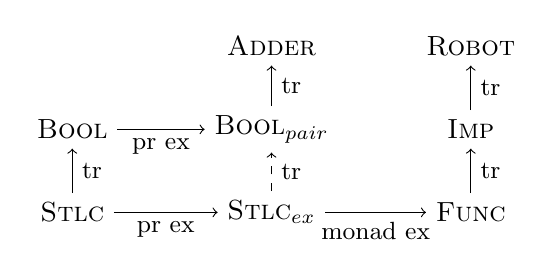
\begin{tikzpicture}[x=6pt,y=3pt,yscale=1,xscale=1]
%uncomment if require: \path (0,300); %set diagram left start at 0, and has height of 300

\node (STLC) at (-2,10) {\textsc{Stlc} };
\node (Bool) at (-2,20) {\textsc{Bool} };
\node (Boolp) at (10,20) {\textsc{Bool}$_\text{pair}$};
\node (Adder) at (10,30) {\textsc{Adder} };
\node (STLCex) at (10,10) {\textsc{Stlc}$_\text{ex}$};
\node (Ref) at (22,10) {\textsc{Func} };
\node (Imp) at (22,20) {\textsc{Imp} };
\node (Robot) at (22,30) {\textsc{Robot} };

\draw[->] (STLC) -> node[right] {\small tr} (Bool); 
\draw[->] (Bool) -> node[below] {\small pr ex} (Boolp);
\draw[->] (STLC) -> node[below] {\small pr ex} (STLCex);
% \draw[->] (STLC) -- node[below] {\small pr ex} (STLC-|STLCex) 
%  -> node[right] {\small tr} (STLCex);
\draw[->] (STLCex) -> node[below] {\small monad ex} (Ref); 
%\draw[->] (Ref) -> node[below] {\small monad ex (IO)} (RefIo);
\draw[->] (Ref) -> node[right] {\small tr} (Imp); 
\draw[->] (Imp) -> node[right] {\small tr} (Robot); 
\draw[->] (Boolp) -> node[right] {\small tr} (Adder); 
\draw[->, dashed] (STLCex) -> node[right] {\small tr} (Boolp); 
\end{tikzpicture}

  \caption{Languages Extended and Specialized from \STLC}
  \label{fig:langs}
\end{figure}

\subsubsection{Language \textsc{Adder}}

Consider that developers would like to
\diwchanged{
develop a DSL based on the \textsc{Bool} language, named \textsc{Adder},
which
}
supports $\<halfa>$ and $\<fulla>$ to simulate digital circuit. For example, in the language \textsc{Adder}, we have
\[ \<halfa>~\<true>~\<false> \Da (\<true>, \<false>). \]
However, they are not easily implemented by translation rules directly, because half-adder and full-adder will get the pair of sum and carry as the results. Pairs are demanded to build compound data structures now. Primitive extensions are used to make the host language support new data types.
In this example, developers add pair and projection to the language, and specify the evaluation (and typing) rules for each newly-defined language construct. Then developers get a new language $\textsc{Bool}_{\text{pair}}$ supporting pairs and projection. With the following translation rules, we can implement the DSL \textsc{Adder} that simulates half-adders and full-adders.
\begin{align*}
\<halfa>~e_1~e_2 & ->_d (e_1~\<xor>~e_2,e_1~\<and>~e_2) \\
\<fulla>~e_1~e_2~e_3 & ->_d (e_1~\<xor>~e_2~\<xor>~e_3, (e_1~\<xor>~e_2)~\<or>~(e_3~\<and>~(e_1~\<xor>~e_2)))
\end{align*}

The evaluation rules of $\<halfa>$, for example, are derived as follows:
\begin{gather*}
\inference{e_1\Da \<true> & e_2\Da \<true>}{\<halfa>~e_1~e_2 \Da (\<false>,\<true>)} \quad
\inference{e_1\Da \<true> & e_2\Da \<false>}{\<halfa>~e_1~e_2 \Da (\<true>,\<false>)} \\[1em]
\inference{e_1\Da \<false> & e_2\Da \<true>}{\<halfa>~e_1~e_2 \Da (\<true>,\<false>)} \quad
\inference{e_1\Da \<false> & e_2\Da \<false>}{\<halfa>~e_1~e_2 \Da (\<false>,\<false>)}
\end{gather*}
% At this time monad has not been introduced. 

%  implementing some languages based on \STLC. 
% Some of these language have been discussed.
% We start with \STLC, a language with lambda calculus and Boolean values.
% From \STLC, we define \textsc{Bool} using translation rules.
% By extending \textsc{Bool} with meta-extensions, we get $\textsc{Bool}_{\text{pair}}$ supporting pairs and projection.
% With two additional translation rules, we implement a DSL \textsc{Adder} that can simulate half adders and full adders.

\subsubsection{Language \textsc{Imp}}

Since we have added a store to \Func, we can now express programs that contain side effects. 
Taking \Func\ as the host language, we want to implement a reference-based imperative language \textsc{Imp}.
In \Func, the declarations and initial values of variables are necessary.
% For example, a legal \textsc{Imp} program and \Func\ program after translation are shown as follows:
For instance, a legal \Func\ program is shown as follows:
\[  \<let>~x=\<ref>~1~\<in>~x:=\ !x+1;\ !x \]
%In contrast, the following program is not permitted but is closer to general IMP programs:
Ideally, we want to write the corresponding DSL program in a more traditional IMP-like syntax:
\[ x:=1;x:=x+1. \]
We discuss why it is impossible to make the syntax of \textsc{Imp} exactly the same as traditional IMP-like language. Moreover, we define some other common language constructs for \textsc{Imp}.
% for convenience.

The declaration in the \textsc{Imp} language is a let-binding in \Func, where what is assigned must be a reference to some expression. In order to simulate the syntax of declaration in common imperative languages, we can define translation rule $\<var>$ as a syntactic sugar:
\[ \<var>~x=e_1; e_2 ->_d \<let>~x=\<ref>~e_1~\<in>~e_2 \]
This semicolon is used as part of the syntax of declaration, to ensure that $x$ is valid in $e_2$.

At first glance, this seems like a perfect translation. However, in an usual assignment statement, the left-hand side is a variable, denotes a location in the store (known as the L-value in the C-world) but any variable at the right-hand side refers to the value stored in it (known as the R-value in the C-world). We cannot distinguish these different occurrences by using translation rules.
% Regretfully, we are not able to simplify this by translation rules, 
As a result, explicit dereferences are required in \textsc{Imp} programs. % A solution is to distinguish such $x$ by the parser, and transform to $!x$ in abstract syntax tree automatically. To prevent confusion, we still write dereferences in the following discussion.

\begin{figure}
  \begin{align*}
    \<var>~x=e_1; e_2 & ->_d \<let>~x=\<ref>~e_1~\<in>~e_2 \\
    \<when>~e_1~e_2 & ->_d \<if>~e_1~e_2~() \\
    e_1 +\!\! = e_2 & ->_d e_1 := !e_1 + e_2 \\
    \<while>~e_1~\<do>~e_2~\<end> & ->_d ((\<fix>~(\lambda f.~\lambda x.~\lambda y.~\<if>~x~\<then>~(y; (f~x~y)_N)~\<else>~()))~e_1~e_2)_N
  \end{align*}
  \caption{Translation Rules for \textsc{Imp}}
  \label{fig:imp}
\end{figure}

Other language constructs in \textsc{Imp} are defined in Fig. \ref{fig:imp}. Note that we define $\<while>$ using the $\<fix>$ construct, because recursively defined translation rules are not allowed. {Note that} the translation rule does not satisfy assumption \ref{asm:tr_abs}, {because} $\<if>$ and sequencing are used in the non-abstract component of lambda abstraction. Using lambda lifting, we get the following two translation rules:
\begin{align*}
    \<body>~e~e_1~e_2 & ->_d \<if>~e_1~\<then>~e_2;(e~e_1~e_2)_N~\<else>~() \\
    \<while>~e_1~\<do>~e_2~\<end> & ->_d ((\<fix>~(\lambda f.~\lambda x.~\lambda y.~\<body>~f~x~y))~e_1~e_2)_N
\end{align*}
Those derived evaluation rules satisfy abstraction property with $\<body>,\<fix> \in \mathcal{S}$, shown in Fig. \ref{fig:while_rule}. 
Note that we do not applied rule of $\<body>$ recursively, since all the constructs in the expression are elements of $\mathcal{S}$.
As an instance of \textsc{Imp}, the following program is implemented to calculate the sum of 1 to 10.
\[ \<var>~n=1;\<var>~sum=0;\<while>~n < 11~\<do>~sum\ +\!\!=\ !n; n\ +\!\!=\ 1;\ !sum~\<end> \]

\begin{figure}
\begin{gather*}
  \inference{e_1 \Da_S \<true> & e_2 \Da_S () & e \Da_S \lambda x.~\lambda y.~e' & [x\mapsto e_1, y\mapsto e_2]e' \Da_S v}{\<body>~e~e_1~e_2 \Da_S v} \\[1em]
  \inference{e_1 \Da_S \<false> }{\<body>~e~e_1~e_2 \Da_S ()} \qquad
  \inference{\<body>~(\<fix>~(\lambda f.~\lambda x.~\lambda y.~\<body>~f~x~y))~e_1~e_2 \Da_S v}{\<while>~e_1~\<do>~e_2~\<end> \Da_S v}
\end{gather*}
    \caption{Derived Evaluation Rule of $\mathit{body}$ and $\mathit{while}$}
    \label{fig:while_rule}
\end{figure}

\subsubsection{Language \textsc{Robot}}

Based on \textsc{Imp}, we implement a DSL named \textsc{Robot}. The language assumes that a robot is located at some \diwchanged{initial coordinate} and users can control its movement or print out its position with commands. 
% In this example, we will emphasize the close property of translation rules. The goal of this language is to achieve simple control of robots in a two-dimensional plane.
A sample program of \text{Robot} is:
\[ \mathit{robot~5~5~\{ up, up, right, whereAmI, left, whereAmI \}} \]
where $\mathit{robot}~5~5~\{...\}$ declares a robot with an \diwchanged{initial coordinate} of $(5,5)$,
and the braces contain a series of commands to be executed on the robot, splitted by a comma.
Commands $\mathit{up},\mathit{right},\mathit{left}$ are used to control the movement of the robot
 and command $\mathit{whereAmI}$ will print current position.

As a natural idea, we \diwchanged{might} record the current position of the robot via the global variables $x$ and $y$. Then each command reads and manipulates global variables, and the comma is defined as sequencing. These language constructs are defined as follows:
\begin{align*}
  \<robot>~e_1~e_2~\{e\} & ->_d \<let>~x=\<ref>~e_1,y=\<ref>~e_2~\<in>~e \\
  e_1,e_2 & ->_d e_1;e_2 \\
  \<left> & ->_d x:=\ !x-1 \\
  \<whereAmI> & ->_d \<print>~!x; \<print>~!y
\end{align*}
where $x$ and $y$ are literal identifiers. \diwchanged{However,} under such definitions, the requirement of closed translation rules is not satisfied. \diwchanged{Because} variables without local bindings cannot be used directly in translation rules, it is necessary to pass the value of the variable as an argument to the language constructs or as an argument to a lambda abstraction. Hence, $\<left>$ should be expressed as
\[ \<left> ->_d λpos. ~(\<fst>~pos)~ \texttt{+=}~ (-1); pos, \]
where $pos$ has type $(\<Rf>~\<int>)\times (\<Rf>~\<int>)$.
Note that $\<left>$ returns $pos$ to keep passing on the ``global'' state.
Then, the comma operator is actually the composition of these functions.
Some other selected translation rules for \textsc{Robot} are given in Fig. \ref{fig:robot}.

\begin{figure}
  \begin{align*}
    \<robot>~e_1~e_2~\{e \} & ->_d e~(\<ref>~e_1,\<ref>~e_2) \\
    e_1,e_2 & ->_d λpos. ~e_2~(e_1~pos) \\
    \<left> & ->_d λpos. ~(\<fst>~pos)~ \texttt{+=}~ (-1); pos \\
    \<whereAmI> & ->_d λpos. ~\<print>~!(\<fst>~pos); \<print>~!(\<snd>~pos); pos
  \end{align*}
  \caption{Translation Rules for \textsc{Robot}}
  \label{fig:robot}
\end{figure}

Don't forget that because they are defined via lambda abstraction, lambda lifting is also necessary.

%%%%%%%%%%%%%%%%%%%%%%%%%%%%%%%%%%%%%%%%%%%%%%%%%%%%%%%%%%%%%%%%%%%%%%%%%%%%%%%%%%%%%%%

\subsection{DSLs on Imperative Host Languages}

Consider that we would like to implement a DSL to simulate finite-state machines, called \textsc{Fsm}.
We simplify the \diwchanged{setting} by using integers to represent states and symbols.
In this section, we will implement a language in which the programs look like this:
\begin{align*}
& \<automata>: \\
& \hspace{1em} \<input> ~ 5\ \{ r~0; r~1; r~0; r~1; r~0 \}; \\[-5pt]
& \hspace{1em} \<exec>\ \{ 0 \xrightarrow{0} 2; 0 \xrightarrow{1} 1; 
 1 \xrightarrow{0} 2; 1 \xrightarrow{1} 1; 
 2 \xrightarrow{0} 2; 2 \xrightarrow{1} 3; 
 3 \xrightarrow{0} 1; 3 \xrightarrow{1} 0; \}; \\
& \hspace{1em} \<enda>;\end{align*}
This machine has 4 states and 2 symbols in the alphabet.
The initial state is 0 (implicitly) and transition rules are defined after keyword $\<exec>$.
We use 5 symbols as input of this automaton declared by $\<input>$, 
and the \diwchanged{evaluation of the} program should tell us the final state.

To implement this, we choose a simplified version of \Cminor{} \cite{cminor} as the host language.
In our problem, we only need to define the main function, so we can ignore \diwchanged{language features} such as the function call stack.
In addition, types and memory models are not our focus. 
Therefore, we assume that only integers are stored in the heap, meaning that the offset of a pointer is fixed.
% In this language, we need to maintain the global memory state and the environment mapping local variables to values.
% Similarly, we use state monad to follow them.
% In addition, incorrect store or load will cause diverging computation, which can be described by maybe monad.
% Through monad transformer, we can combine the above two monads as one monad, denoted by $m$.

The DSL program will be translated into the execution of the main function.
In \Cminor{}, a function is defined by a list of parameters (null for main function), 
 a list of local variables, and a body statement.
Defining variables in the body is not allowed.
Therefore, to provide the translation rules for the DSL,
we need to identify the local variables that will be used in \textsc{Fsm}.
% The language construct $\<automata>$ in \textsc{Fsm}, which will be translated into a \Cminor{} program,
% must declare these local variables.
The translation rule of $\<automata>$ is defined as follows:
\[ \<automata>:~stmt ->_d \texttt{main() \{ var n,syms,i,st; $stmt$ \}} \]
where $stmt$ is the body of main function; 
$n$ is the number of input symbols; 
$syms$ is the pointer pointing to the first cell of input symbols;
$st$ is current state;
and $i$ is auxiliary variable for iteration.

The language constructs $\<input>$ and $r$ are used to record the input symbols.
The $\<input>$ \diwchanged{construct} first initializes local variable $n$ and $i$, and then allocates the requested size.
After that, $r$ is used to store the inputs.
The translation rules of $\<input>$ and $r$ are defined as:
\begin{align*}
  \<input>~expr~stmt & ->_d \texttt{n := }expr\texttt{; i := 0; syms := malloc(n); } stmt \\
  r~expr & ->_d \texttt{[syms + i] := } expr \texttt{; i := i + 1;}
\end{align*}
In RHS, statements include assignment to local variable (with shape \texttt{ident := expr}, memory stores (with shape \texttt{[$expr$] := $expr$}) and sequencing.
Expressions include reading local variables, constants, \diwchanged{binary} operations, and function calls.
In \Cminor{}\ , \texttt{malloc} is seen as an external function, while we use it as a primitive operation, 
which takes the size as argument and returns the address of a
\diwchanged{newly allocated memory block with the requested size}.

The \textsc{FSM} processes input through language construct $\<exec>$. 
It repeatedly changes the state based on the current input until all input characters are consumed.
The body of $\<exec>$ consists of a list of transfer rules and each of them will be translated into an \texttt{if} statement.
If one of the rule is matched, there should be a \texttt{continue}.
And if there is no rule that can be matched, the state will be set as $-1$ and the loop should exit through \texttt{break}. 
In \Cminor{}, only infinite looping is introduced.
And \texttt{break} and \texttt{continue} are implemented with blocks and \texttt{exit} statements.
We use $\texttt{exit}~n$ to leave $(n+1)$ enclosing blocks.
For example, in \Cminor{}, $\texttt{while}~e~s$ is written as 
\[ \texttt{block \{ loop \{ if !$e$ then exit 0; block \{ $s$ \} \}\}}. \]
Note that the braces here are used to enclose a group of statements connected by sequence, 
while a block is used with the \texttt{block} language construct.
In $s$, if there are no nested blocks, \texttt{continue} can be written as \texttt{exit 0} and \texttt{break} \diwchanged{can be written as} \texttt{exit 1}.
Based on the above discussion, we can define the following translation rules:
\begin{align*}
    \<exec>~stmt & ->_d \texttt{i := 0; block \{ loop \{ if (i == n) exit 0; } \\ 
    & \qquad\qquad \texttt{block \{}~stmt~\texttt{; st := -1; exit 1; \}\}\} }  \\
    expr_1 \xrightarrow{expr} expr_2 & ->_d \texttt{if (st == } expr_1 \texttt{ \&\& load (syms + i) == } expr \texttt{) \{} \\
    & \qquad\qquad \texttt{st := } expr_2 \texttt{; i := i + 1; exit 0; \}}
\end{align*}

Finally, $\<enda>$ is used to print the final state.
\[ \<enda> ->_d \texttt{print(st); return 0;} \]
where \texttt{print} is an external function in \Cminor{} and \texttt{return} statement will finish the function execution.

Next, we will discuss the semantics of \Cminor{}.
We use a monad to describe the changes in the global heap and local environment.
Due to diverging computations caused by incorrect storage and retrieval, 
and the \diwchanged{potential} use of undefined variables, 
we also need to introduce the maybe monad.
We combine the above two monads with the I/O monad using a monad transformer and denote \diwchanged{the combined monad} as $m$.

The evaluation of an expression $expr \Da_m val$ does not cause changes in the environment or memory, 
but it may read the value of variables or pointed-to values of pointers from the state.
Statements evaluate to \textit{outcomes} $stmt \Da_m out$, indicating how afterwards execute. 
There are three types of outcomes: \texttt{norm} (for normal, continuing in sequence), $\texttt{ex}~n$ (for exit, terminating the $n+1$ enclosing blocks), $\texttt{ret}~val$ (for return).
Some evaluation rules of expressions and statements are shown in Fig. \ref{fig:cminor}.
One thing to note here is the \texttt{loop} construct.
By using $later$, We transform the recursion in the evaluation rule of the \texttt{loop} construct into a meta-function call to satisfy assumption \ref{asm:host_abs}.
Clearly, the meta-function $later(stmt)$ returns the evaluation result of $stmt$.
Furthermore, \diwchanged{because} $stmt$ is used as an argument in the meta-function, 
it is a non-abstract component of \texttt{loop $stmt$}.
All these evaluation rules and meta-functions obey the assumptions.

\begin{figure}

\addtolength{\jot}{5pt}
\begin{gather*}
\noalign{\raggedright \hspace{2em} Expression: $expr \Da_m val$}
\inference{\mathit{get}(x) =>_m val}{x \Da_m val} \quad
\inference{expr\Da_m addr & \mathit{load}(addr)=>_m val }{\texttt{load}~expr \Da_m val } \\
\noalign{\raggedright \hspace{2em} Statement: $stmt \Da_m out$}
\inference{ expr\Da_m val & update(x, val)}{x := expr \Da_m \texttt{norm} } \\
\inference{ expr_1\Da_m addr & expr_2 \Da_m val & store(addr, val)}{ [expr_1] := expr_2 \Da_m \texttt{norm} } \\
\inference{ stmt_1\Da_m \texttt{norm} & stmt_2\Da_m out }{stmt_1;stmt_2 \Da_m out } \quad
\inference{ stmt_1\Da_m out & out \ne \texttt{norm} }{stmt_1;stmt_2 \Da_m out } \\
\inference{ stmt \Da_m \texttt{norm} & later(\texttt{loop}~stmt) =>_m out }{ \texttt{loop}~stmt \Da_m out } \quad
\inference{ stmt \Da_m out & out \ne \texttt{norm} }{ \texttt{loop}~stmt \Da_m out } \\
\inference{ stmt \Da_m \texttt{ex}~0 }{ \texttt{block}~stmt \Da_m \texttt{norm} } \quad
\inference{ stmt \Da_m \texttt{ex}~n }{ \texttt{block}~stmt \Da_m \texttt{ex}~(n-1) } \\
\inference{ stmt \Da_m out & out \ne \texttt{ex}~n }{ \texttt{block}~stmt \Da_m out } \quad
\inference{}{ \texttt{exit}~n \Da_m \texttt{ex}~n } \quad
\inference{ expr \Da_m val }{ \texttt{return}~expr \Da_m \texttt{ret}~val } \\
\noalign{\raggedright \hspace{2em} Main Function: $\mathit{func} \Da_m val$}
\inference{ \mathit{newEnv}(vars) & stmt \Da_m \texttt{ret}~val }{\texttt{main() \{ var $vars$; $stmt$ \} } \Da_m val }
\end{gather*} 

\caption{Selected Evaluation Rules of \Cminor{}}
\label{fig:cminor}
\end{figure}

For the translation rules, we need to show that they satisfy our closed translation requirement.
In \Cminor{}, all variable assignments and reads are done through meta-functions, 
which means that undefined variables will fail at run-time of the meta-function.
In the derived evaluation rules, variables can be read dynamically.
Hence, in the translation rules, it is not necessary to perform local binding for variables to achieve correct semantics lifting.
But correspondingly, hygiene cannot be guaranteed as a result.
To satisfy assumption \ref{asm:tr_abs}, \texttt{exec} needs to be split into two translation rules:
\begin{align*}
\texttt{step}~stmt & ->_d \texttt{if (i == n) exit 0; block \{}~stmt~\texttt{; st := -1; exit 1; \} }  \\
\<exec>~stmt & ->_d \texttt{i := 0; block \{ loop \{ \texttt{step}~stmt \}\} }  \\
\end{align*}
Their semantics can be statically derived and will not be elaborated here.

% \begin{figure}
%     \centering
%     \begin{verbatim}
%     int main() { 
%       var n, syms, i, st; 
%       n := 5; i := 0; syms = malloc(5);  // input 5
%       [syms + i] := 0; i := i + 1;  // r 0
%       [syms + i] := 1; i := i + 1;  // r 1
%       ...
%       i := 0; block { loop {  // exec
%         if (i == n) exit 0; block {
%           if (st == 0 && load (syms + i) == 0) {
%             st := 2;
%             i := i + 1;
%             exit 0;
%           }
%           ...
%           st := -1; exit 1;
%         }
%       } }
%       print(st); return 0;
%     }
%     \end{verbatim}
%     \caption{Caption}
%     \label{fig:my_label}
% \end{figure}


% From another dimension, we start with meta-extensions on \STLC.
% Language constructs pairs, sums, fixpoints and lists,
%  introduced in Chapter 11 of Types and Programming Languages\cite{tapl} are tested.
% And let bindings and ascription are implemented by translation rules.
% We name the new language as \STLCex.
% In this language, we will talk about the impact of fixpoints on abstraction.

% Then, we introduce reference and I/O by monad extension, getting \textsc{Ref}.
% Taking \textsc{Ref} as the host language,
%  we implement an imperative language \textsc{Imp}.

% The point we should care about in \textsc{Imp} is that,
%  recursive translation rules are declared in $\<while>$.
% As an extension of our framework,
%  we will discuss weak-abstraction semantics derivation.
%
% After that, we make \textsc{Ref} support I/O, getting \RefIO.
% Based on \textsc{Imp}, we implement a DSL named \textsc{Robot}.
% The language assumes that a robot is located at some starting coordinates,
%  and users can control its movement, or print out its position with commands.
% In this example, We will talk about how to access ``global variables'' in the translation rules.

% \subsection{\STLCex: Fixpoint}\label{sec:fix}

% Fixpoint is a common approach to implement recursion in functional programming language.
% As a primitive language construct, the evaluation rule and typing rule of $\<fix>$ are specified:
% \begin{align*}
%   \ctr{Fix}{ \<fix>~e} & \cqq \Let{λx\!:\!t.e_1}{\EE{e}} \EE{e_1[\<fix>~(λx\!:\!t.e_1)/x]}
%   % \TT{\<fix>~e} & \cqq \TT{e}:(t_1->t_2\mid t_1=t_2 |> t_1). 
% \end{align*}

% Since an expression with substituion are evaluated,
%  the evaluation rule is not structural.
% And as mentioned above, nonstructural evaluation rule should be considered how to maintain abstraction.
% % In fact, thanks to lambda lifting and the existing discussion on substitution, fixpoint is easy to solve.
% % However, unfolding according to the rules of $\<fix>$ leads to non-termination of the algorithm.
% We assume that fix can be preserved in the DSL--for a language that contains recursion is straightforward.
% We add the following rule to the $\dd$:
% \[ \dd(\HH{\<fix>~\mexp}) = \Let{λx\!:\!t.e_1}{\dd(\HH{\mexp})} \HH{\<fix>~(λx\!:\!t.e_1)} \]
% where we do not expand the substitution with fixpoint resursively.
% The above rule is equivalent to the extended rule in Section \ref{sec:alg-ex}, but the $\<fix>$ is kept in the rule for readability.

% \begin{example}
% \[ \<iseven> => \<fix>~(λie\!:\!int->bool.~λx\!:\!int.~\<if>~(x=lit~0)~\<true>~(\<if>~(x=lit~1)~\<false>~(ie~(x-lit~2)))) \]
  
% The first step is lambda lifting. The following translation rules are generated.
% \begin{align*}
%   \<iseven>'~e_1~e_2 & => \<if>~(e_2=lit~0)~\<true>~(\<if>~(e_2=lit~1)~\<false>~(e_1~(e_2-lit~2))) \\
%   \<iseven> & => \<fix>~(λie\!:\!int->bool.~λx\!:\!int.~\<iseven>'~ie~x)
% \end{align*}

% The evaluation rules of language constructs used by $\<iseven>'$ all have structural semantics.
% So the evaluation rule of $\<iseven>'$ is also structural.
% The evaluation rule of $\<iseven>$ can be derived by:
% \begin{align*}
%   & \ctr{IsEven}{\<iseven>} \\
%   \cqq~ & \dhl{\HH{\<fix>~(λie\!:\!int->bool.~λx\!:\!int.~\<iseven>'~ie~x)}} \\
%   =~ & \Let{λx'\!:\!t.e}{\dhl{\HH{λie\!:\!int->bool.~λx\!:\!int.~\<iseven>'~ie~x}}} \HH{\<fix>~(λx':t.e)} \\
%   =~ & \HH{\<fix>~(λie\!:\!int->bool.~λx\!:\!int.~\<iseven>'~ie~x)}
% \end{align*}
% Because of lambda lifting, $\<iseven>'$ is a DSL construct. The abstraction property holds.
% \end{example}



% \subsection{\textsc{Imp}: Recursive Translation Rules}\label{sec:while}

% Our \textsc{Imp} language is defined by translation rules based on \textsc{Ref},
%  which means the use of variables should be reference-based.
% Therefore, the syntax of \textsc{Imp} here is slightly different from the general language.
% First, the declarations and initial values of variables are necessary.
% For example, a legal \textsc{Imp} program is
% \[ \<let>~x=\<ref>~1~\<in>~x:=!x+1; !x \]
% And $x:=1;x:=x+1;x$ is not permitted for $x$ not in scope.
% Also, we find that what is assigned in the declaration must be a reference to some expression.
% In order to simulate the syntax of declaration in common imperative language,
%  we can define syntactic sugar $\<var>$ shown in Fig. \ref{fig:imp}.
% The semicolon is used as part of the syntax of the declaration, to ensure that $x$ is valid in $e_2$.

% Second, in \textsc{Imp}, the left-hand side of an assignment must be a variable
%  and the any variable at right-hand side refers to the value stored in it (a location).
% Regretfully, we are not able to simplify this by translation rules,
%  and explicit dereferences are essential.
% A solution is to distinguish such $x$ by the parser, and transform to $!x$ in abstract syntax tree automatically.
% We still write dereferences in the following discussion.

% \begin{figure}
%   \begin{align*}
%     \<var>~x=e_1; e_2 & => \<let>~x=\<ref>~e_1~\<in>~e_2 \\
%     \<when>~e_1~e_2 & => \<if>~e_1~e_2~() \\
%     e_1 +\!\! = e_2 & => e_1 := !e_1 + e_2 \\
%     \<while>~e_1~\<do>~e_2~\<end> & => \<if>~e_1~(e_2; \<while>~e_1~\<do>~e_2~\<end>)~()
%   \end{align*}
%   \caption{Translation Rules for \textsc{Imp}}
%   \label{fig:imp}
% \end{figure}

% Some other common language constructs in \textsc{Imp} are defined in Fig. \ref{fig:imp}.
% But $\<while>$, whose definition does not satisfy requirement \ref{req:no-recursion}, is our concern.
% By the algorithm extension of Section \ref{sec:alg-ex}, we have
% \begin{align*}
%   & \ctr{While}{\<while>~e_1~\<do>~e_2~\<end>} \\ 
%   \cqq~~ & \dhl{\EE{\<if>~e_1~(e_2; \<while>~e_1~\<do>~e_2~\<end>)~()}} \\
%   =~~ & \EE{e_1}:\branch{
%         \<true> |> \Let{()}{\EE{e_2}} \dhl{\EE{\<while>~e_1~\<do>~e_2~\<end>}} \\&
%         \<false> |> ()
%     } \\
%   =~~ & \EE{e_1}:\branch{
%       \<true> |> \Let{()}{\EE{e_2}} \EE{\<while>~e_1~\<do>~e_2~\<end>} \\&
%       \<false> |> ()
%   }
% \end{align*}
% Consider that we discard this step of expansion, the evaluation rule of $\<while>$ can be derived as follows, 
%  which is not structural but correct:
% \[ 
%   \ctr{While}{\<while>~e_1~\<do>~e_2~\<end>} \cqq \EE{e_1}:\branch{
%     \<true> |> \Let{()}{\EE{e_2}} \EE{\<while>~e_1~\<do>~e_2~\<end>} \\&
%     \<false> |> ()
%   } 
% \]
% Because $\<while>$ itself is a language construct in the DSL,
%  we can think of it as satisfying abstraction if we keep it in the evaluation rule.

% The more serious problem is the type derivation.
% It is reasonable that $\<while>$ has a recursive evaluation,
%  but the typing of $\<while>$ should not be.
% If the above approach is applied, an error typing rule is generated:
% \begin{align*}
%   \TT{\<while>~e_1~\<do>~e_2~\<end>} \cqq~
%   & \Let{\<bool>}{\TT{e_1}} \Let{\<unit>}{\TT{e_2}} \\
%   & \Let{t_2}{\TT{\<while>~e_1~\<do>~e_2~\<end>}} \<unit>:(t_3 \mid t_2=t_3 |> t_2)
% \end{align*}
% In this instance, the typing rule must be specified manually.

% More problem arise when \textsc{Imp} is used as a host language.
% When a language construct is translated to $\<while>$,
%  abstraction is difficult to guarantee.
% For example, $\<for>$ can be defined as follows, but we cannot derive an evaluation rule without $\<while>$.
% \[ \<for>~(e_1;e_2;e_3)~\<do>~e_4 => e_1;\<while>~e_2~\<do>~(e_4;e_3)~\<end> \]



% \subsection{\textsc{Robot}: Access to Global Variables}

% The goal of this language is to achieve simple control of robots in a two-dimensional plane.
% A sample program of \text{Robot} is:
% \[ \mathit{robot~5~5~\{ up, up, right, whereAmI, left, whereAmI \}} \]
% where $\mathit{robot}~5~5\{...\}$ declares a robot with a starting point of $(5,5)$,
% and the braces contain a series of commands to be executed on the robot, splitted by comma.
% Some commands are used to control the movement of the robot,
%  and command $\mathit{whereAmI}$ will print current position.

% As a natural idea, we record the current position of the robot via the global variables $x$ and $y$.
% Then each command reads and manipulates global variables,
%  and comma is defined as sequencing.
% These language constructs are defined as follows:
% \begin{align*}
%   \<robot>~e_1~e_2~\{e\} & => \<let>~x=\<ref>~e_1,y=\<ref>~e_2~\<in>~e \\
%   e_1,e_2 & => e_1;e_2 \\
%   \<left> & => x:=\ !x-1 \\
%   \<whereAmI> & => \<print>~!x; \<print>~!y
% \end{align*}
% where $x$ and $y$ are literal identifiers.
% But requirement \ref{req:close} is not satisfied.
% Since variables without local bindings cannot be used directly in translation rules,
%  it is necessary to pass the value of the variable as an argument to the language constructs or as an argument to a lambda abstraction.
% Hence, $\<left>$ can be expressed as
% \[ \<left> => λpos:(\<Rf>~\<int>)\times (\<Rf>~\<int>). ~(\<fst>~pos)~ \texttt{-=}~ 1; pos \]
% Note that $\<left>$ returns $pos$ to keep passing on the ``global'' state.
% Then, the comma operator is actually the composition of the functions.
% Some selected translation rules for \textsc{Robot} are given in Fig. \ref{fig:robot}.

% \begin{figure}
%   \begin{align*}
%     \<robot>~e_1~e_2~\{e\} & => e~(\<ref>~e_1,\<ref>~e_2) \\
%     e_1,e_2 & => λpos:(\<Rf>~\<int>)\times (\<Rf>~\<int>). ~e_2~(e_1~pos) \\
%     \<left> & => λpos:(\<Rf>~\<int>)\times (\<Rf>~\<int>). ~(\<fst>~pos)~ \texttt{-=}~ 1; pos \\
%     % \<right> & => λpos:(\<Rf>~\<int>)\times (\<Rf>~\<int>). ~(\<fst>~pos)~ \texttt{+=}~ 1; pos \\
%     % \<down> & => λpos:(\<Rf>~\<int>)\times (\<Rf>~\<int>). ~(\<snd>~pos)~ \texttt{-=}~ 1; pos \\
%     % \<up> & => λpos:(\<Rf>~\<int>)\times (\<Rf>~\<int>). ~(\<snd>~pos)~ \texttt{+=}~ 1; pos \\
%     \<whereAmI> & => λpos:(\<Rf>~\<int>)\times (\<Rf>~\<int>). \<print>~!(\<snd>~pos); \<print>~!(\<fst>~pos); pos
%   \end{align*}
%   \caption{Translation Rules for \textsc{Robot}}
%   \label{fig:robot}
% \end{figure}


\section{Related Work}

Our work on language lifting for DSL is related to the work on meta-language design, DSL implementation and abstraction maintenance.

\paragraph{Abstraction Maintenance.}
For evaluation, the main related work is how to correspond the transformed program back to the source in optimization and debugging \cite{resugar,abs-1,abs-2,abs-3}.
Resugaring maintains abstraction dynamically and provides the evaluation sequences to users.
In order to illustrate the correctness of the evaluation sequences, resugaring proposes two properties: emulation and coverage \cite{resugar}.
We can only give the evaluation rules of the DSL now and 
 will consider giving the evaluation sequences holding these properties as future work.
% As far as we are aware, our framework is the first one to derive semantics for DSL and make it standalone.
For typing, \cite{infer-types,type-sound,type-sound-1} have done pretty much work on statically deriving typing rules and guaranteeing the soundness of type system for syntactic sugar.
The type derivation in our work is a natural application of the rule derivation
 and is not as competent as related work and is not our main contribution.

\paragraph{Meta-language Design.}
Our meta-language is designed built upon the skeletal semantics \cite{skeleton},
 which can capture the behaviour of a language construct in a single rule.
By providing different interpretation,
 the skeletal semantics can build consistency between abstract and concrete interpretations.
It has similars structure in behaviour description,
 but there are sharp differences from ours:
(1) We use two rules to describe evaluation and typing respectively, instead of a single rule in skeleton;
(2) Different from in skeleton, where a filter has various definition in different interpretation, 
 there is only one interpretation in our meta-language and the meta-functions are pre-defined.
(3) We permit the use of monad in computation to cover side effects.
K-framework \cite{K-framework}, Ott \cite{Ott} also allow users to define the semantics formally.
The semantics defined in K is rewrite-based, using matching logic.
For ease to use, K provides an executable interpreter and a program verifier.
Ott provides a meta-language to write semantics concisely and compiles these definition to Coq code.
The focus of these tools is on the formalization and verification of the language itself.
And our meta-language design concentrates on the feasibility of language lifting.

\paragraph{DSL Implementation.}
There is a long history of DSL implementation \cite{MartinDSL,when-how-dsl}.
Our translation rules are essentially similar to macros and syntactic sugar.
Distinguish from selecting the appropriate host language based on the DSL design,
 we put more emphasis on the gradual expansion of the host language to append required features \cite{MoggiMeta}.
The expression problem \cite{expr-problem} is orthogonal to our problem.
The goal of expression problem is the extensibility both in data structure and interpretations,
 keeping the existing modules intact.
Instead, we directly expand the existing data structure definition for translation rules,
 which is not allowed in the expression problem.
Our approach is on top of the host language and is neither deep or shallow embedding.

\section{Conclusion}

In this paper, we propose a \diwchanged{systematic framework} to lift semantics for domain-specific languages.
We present a \diwchanged{reasonable} set of assumptions to ensure that semantics lifting maintains correctness and satisfies abstraction.
These assumptions are related to the meta-functions, host-language semantics, and translation rules.
We have proved the correctness and abstraction of the semantics-lifting algorithm under such assumptions.
Following this idea, we implement the tool Osazone, which is shown to be \diwchanged{flexible, effective, and practical} to develop DSLs.
Osazone \diwchanged{provides} a meta-language to describe the evaluation rules of \diwchanged{host languages}.
Based on a host language, users can extend the host language to support new vocabularies and language features,
 as well as specify the DSL constructs by translation rules.
As case studies, we take a functional language and a imperative language as host languages and implement DSLs based on these two languages through translation rules. We show how these languages are implemented and illustrate that meta-functions, host languages, and translation rules we used meeet our assumptions. Eventually, we obtain correct, abstract semantics for DSLs.
% \diw{Add some experimental highlights}.

\bibliographystyle{ACM-Reference-Format}
\bibliography{ref.bib}

% \appendix
% \section{Proofs}

\subsection{Proof of Lemma \ref{lemma:sig-bone}}

\begin{lemmaapp}
  Support $\cb$ is a closed bone. Then:
  \[ \cb \rr{X} v \quad\miff\quad \dd(\cb) \rr{X} v. \]
\end{lemmaapp}

\begin{proof}
  By induction on a derivation of $\cb \rr{X} v$. 
  The \textsc{Expression} and \textsc{Filter} cases are immediate, since $\dd(\cb)=\cb$.
  The other cases are shown as follows:

  Case \textsc{Hook}: let $\cb=\EE{e}$, where $e$ is a closed expression.
  We consider each case separately according to $e$:
  \begin{itemize}
    \item $e$ is a base expression: $\dd(b)=b$;
    \item $e=c~\cexp_1\cdots \cexp_n$: we have $\EE{e} \rr{X} v$, iff $L[e] \rr{X} v$.
      Furthermore, according to the definition of $\dd$, 
      we can find an environment $Σ$ and a rule $\EE{\mexp}\cqq b_1$ in $L$, such that $Σ(\mexp) = e$, $\dd(\EE{e})=\dd(Σ(b_1))$.
      According to the definition, $Σ(b_1)=L[e]$.
      Then $\dd(\EE{e})=\dd(L[e])$.
      Since $e$ is a closed variable, $Σ(b_1)$ is a closed bone.
      By the induction hypothesis, $L[e]\rr{X} v$ iff $\dd(L[e])\rr{X} v$.
      Then, $\EE{e}\rr{X} v$, iff $\dd(\EE{e})\rr{X} v$.
  \end{itemize}

  Case \textsc{LetIn}: let $b=\Let{pat}{b_1} b_2$.
    Then $b\rr{X} v$, iff the following judgements are satisfied:  
    \[ b_1\rr{X_1}v_1 \quad Σ=match(pat,v_1) \quad Σ(b_2)\rr{X_2}v_2 \quad X=X_1;X_2, \]
     where $Σ(b_2)$ is a closed bone.
    By the induction hypothesis and Lemma \ref{lemma:del-sig}, we have
    \begin{align*}
      b_1\rr{X_1}v_1    & \quad\miff\quad \dd(b_1)\rr{X_1} v_1, \\
      Σ(b_2)\rr{X_2}v_2 & \quad\miff\quad Σ(\dd(b_2))\rr{X_2}v_2
    \end{align*} 
    Therefore, we can apply rule \textsc{LetIn} to conclude
    \[ \Let{pat}{\dd(b_1)} \dd(b_2) \rr{X} v \]
    whose left-hand side equals to $\dd(b)$.

  Case \textsc{Branch}: Similar.
\end{proof}


\end{document}
\endinput
